% documentclass: article used for scientific journals, short reports, program documentation, etc
% options: fontsize 11, generate document for double sided printing, a4-paper
\documentclass[12pt, twoside, a4paper, fleqn]{article}

% package for changing page layout
\usepackage{geometry}
\geometry{a4paper, lmargin=40mm, rmargin=45mm, tmargin=40mm, bmargin=45mm}
% set indentation
\setlength{\parindent}{1em}
% set factor for line spacing
% \linespread{1.0}\selectfont
% set (dynamic) additional line spacing
% \setlength{\parskip}{1ex plus 0.5ex minus 0.3ex}

% rigorous formatting (not too much hyphens)
% \fussy
% \sloppy

% package for changing page layout (used to indent whole paragraphs with adjustwidth)
\usepackage{changepage}

% input encoding for special characters (e.g. ä,ü,ö,ß), only for non english text
% options: utf8 as encoding standard, latin1
\usepackage[utf8]{inputenc}
% package for font encoding
\usepackage[T1]{fontenc}
% package for changing used language (especially for more than one language)
% options: ngerman (new spelling) or default: english
\usepackage[ngerman]{babel}
% package for times font
% \usepackage{times}
% package for latin modern fonts
\usepackage{lmodern}

% package for math symbols, functions and environments from ams(american mathematical society)
\usepackage{amsmath}
\usepackage{mathtools}
% package for extended symbols from ams
\usepackage{amssymb}
% package for math black board symbols (e.g. R,Q,Z,...)
\usepackage{bbm}
% package used for calligraphic math symbols
\usepackage{mathrsfs}
% package for extended symbols from stmaryrd(st mary road)
\usepackage{stmaryrd}
% package for more math blackboard symbols
\usepackage{dsfont}

% pack­age im­ple­ments scal­ing of the math ex­ten­sion font cmex; used for scaling math signs
\usepackage{exscale}

% package for including extern graphics plus scaling and rotating
\usepackage{graphicx}
%package for positioning figures
\usepackage{float}
% package for changing color of font and paper
% options: using names of default colors (e.g red, black)
% \usepackage[usenames]{color}
\usepackage[dvipsnames]{xcolor}
\definecolor{shadecolor}{gray}{0.9}
% package for customising captions
\usepackage[footnotesize, hang]{caption}
% package for customising enumerations (e.g. axioms)
\usepackage{enumitem}
% calc package reimplements \setcounter, \addtocounter, \setlength and \addtolength: commands now accept an infix notation expression
\usepackage{calc}
% package for creating framed, shaded, or differently highlighted regions that can break across pages; environments: framed, oframed, shaded, shaded*, snugshade, snugshade*, leftbar, titled-frame
\usepackage{framed}
% package for creating custom "list of"
% options: titles: do not intefere with standard headings for "list of"
\usepackage[titles]{tocloft}
% change enumeration style of equations
% \renewcommand\theequation{\thesection.\arabic{equation}}


% provides \ifthenelse command
\usepackage{ifthen}
% extra commands for if-conditions (e.g. \isempty)
\usepackage{xifthen}

% init list of math for definitions and theorems
\newcommand{\listofmathcall}{Verzeichnis der Definitionen und Sätze}
\newlistof{math}{mathlist}{\listofmathcall}
% add parentheses around argument
\newcommand{\parent}[1]{ \ifx&#1&\else (#1) \fi }
\definecolor{mathdefback}{rgb}{0.95,0.95,0.98}
% unnumerated mathematical definition environment definiton
\newenvironment{mathdef*}[2]{
	\medskip
	\begin{tcolorbox}[colback=mathdefback, boxrule=0.5pt, colframe=black, boxsep=0pt, enhanced jigsaw, breakable, arc=3pt]
	\noindent
	{ \fontfamily{ppl}\selectfont \textbf{\textsc{#1:}} } ~ #2 
	\par \hfill\\ 
	\fontfamily{lmr}\selectfont \itshape
}{
	\end{tcolorbox}
	\medskip
}
% definitions for numerated mathematical definition environment
\newcounter{mathdefc}[section]
\newcommand*{\mathdefnum}{\thesection.\arabic{mathdefc}}
\renewcommand{\themathdefc}{\mathdefnum}
\newenvironment{mathdef}[2]{
	\refstepcounter{mathdefc}
	\addcontentsline{mathlist}{figure}{\protect{\numberline{\mathdefnum}#1 ~ #2}}
	\begin{mathdef*}{#1 \mathdefnum}{#2}
}{
	\end{mathdef*}
}
% standard mathdef calls
\newcommand{\definitioncall}{Definition}
\newenvironment{definition*}[1][]{ \begin{mathdef*}{\definitioncall}{\parent{#1}} }{ \end{mathdef*} }
\newenvironment{definition}[1][]{ \begin{mathdef}{\definitioncall}{\parent{#1}} }{ \end{mathdef} }

\definecolor{maththeoremframe}{rgb}{0.7,0.7,0.73}

% unnumerated theorem environment definition
\newenvironment{maththeorem*}[2]{
	\medskip
	\begin{tcolorbox}[boxrule=0pt, leftrule=2.5pt, arc=2pt, colback=white, colframe=maththeoremframe, enhanced jigsaw, breakable, vfill before first, top=0mm, bottom=0mm, left=2mm, right=0mm, boxsep=1mm]
	\noindent
	{ \fontfamily{ppl}\selectfont \textbf{\textsc{#1:}} } ~ #2
	\par \hfill\\ 
	\fontfamily{lmr} \fontshape{it} \selectfont
}{ 
	\end{tcolorbox}
	\medskip
}
% definitions for numerated theorem environment
\newcounter{maththeoremc}[section]
\newcommand*\maththeoremnum{\thesection.\arabic{maththeoremc}}
\renewcommand{\themaththeoremc}{\maththeoremnum}
\newenvironment{maththeorem}[2]{
	\refstepcounter{maththeoremc}
	\addcontentsline{mathlist}{figure}{\protect{\qquad\numberline{\maththeoremnum}#1 ~ #2}}
	\begin{maththeorem*}{#1 \maththeoremnum}{#2}
}{
	\end{maththeorem*}
}
% standard maththeorem calls
\newcommand{\theoremcall}{Theorem}
\newenvironment{theorem*}[1][]{ \begin{maththeorem*}{\theoremcall}{\parent{#1}} }{ \end{maththeorem*} }
\newenvironment{theorem}[1][]{ \begin{maththeorem}{\theoremcall}{\parent{#1}} }{ \end{maththeorem} }
\newcommand{\lemmacall}{Lemma}
\newenvironment{lemma*}[1][]{ \begin{maththeorem*}{\lemmacall}{\parent{#1}} }{ \end{maththeorem*} }
\newenvironment{lemma}[1][]{ \begin{maththeorem}{\lemmacall}{\parent{#1}} }{ \end{maththeorem} }
\newcommand{\propositioncall}{Proposition}
\newenvironment{proposition*}[1][]{ \begin{maththeorem*}{\propositioncall}{\parent{#1}} }{ \end{maththeorem*} }
\newenvironment{proposition}[1][]{ \begin{maththeorem}{\propositioncall}{\parent{#1}} }{ \end{maththeorem} }
\newcommand{\corollarycall}{Korollar}
\newenvironment{corollary*}[1][]{ \begin{maththeorem*}{\corollarycall}{\parent{#1}} }{ \end{maththeorem*} }
\newenvironment{corollary}[1][]{ \begin{maththeorem}{\corollarycall}{\parent{#1}} }{ \end{maththeorem} }
% q.e.d. definition
\newcommand{\qed}{ \par \hfill \fontfamily{lmr} \fontshape{it} \selectfont \mbox{q.e.d.} \\}
\newcommand{\qedbox}{ \hfill $\Box$ }
% proof environment definition for theorems
\newenvironment{mathproof}[2]{
	% \par\hfill\\
	\medskip
	% \noindent
	% \par
	% { \fontfamily{ppl}\selectfont \small \textsc{#1:} } ~ \parent{#2} \smallskip\\
	% \begin{adjustwidth}{1em}{}
	\begin{tcolorbox}[title= { \fontfamily{ppl}\selectfont \small \textsc{#1:} } ~ \parent{#2}, boxrule=0pt, colback=white, colframe=white, coltitle=black, breakable, boxsep=0mm, top=2mm, bottom=0mm, right=0mm, left=0mm, before upper={\parindent1em}]%
	\normalfont
	\small
}{ 
	\end{tcolorbox}
	% \end{adjustwidth} 
	% \qedbox
	\medskip
}
% standard mathproof calls
\newcommand{\proofcall}{Beweis}
\newenvironment{proof}[1][]{ \begin{mathproof}{\textbf{\proofcall}}{#1} }{ \qedbox \end{mathproof} }
\newcommand{\proofideacall}{Beweisidee}
\newenvironment{proofidea}[1][]{ \begin{mathproof}{\proofideacall}{#1} }{ \end{mathproof} }
\newcommand{\examplecall}{Beispiel}
\newenvironment{example}[1][]{ \begin{mathproof}{\examplecall}{#1} }{ \end{mathproof} }

% fast font types
\newcommand{\m}[1]{\mathrm{#1}}
\newcommand{\s}[1]{\mathcal{#1}}


% define
\newcommand{\define}{\coloneqq}
% define sign from the right
\newcommand{\definedby}{\eqqcolon}
% function
\newcommand{\func}[3]{#1\colon#2\to#3}


% brackets
% curly brackets
\newcommand{\curlb}[1]{\left\{ #1 \right\}}
% box brackets
\newcommand{\boxb}[1]{\left[ #1 \right]}
% parentheses/curved brackets
\newcommand{\curvb}[1]{\left( #1 \right)}
% angle brackets
\newcommand{\angleb}[1]{\left\langle #1 \right\rangle}
% floor brackets
\newcommand{\floorb}[1]{\left\lfloor #1 \right\rfloor}
% ceil brackets
\newcommand{\ceilb}[1]{\left\lceil #1 \right\rceil}


% symbols for sets
% create sets
% \newcommand{\set}[2][]{ \curlb{#2 \ifx&#1&\else \enspace\middle\vert\enspace #1 \fi} }
\newcommand{\set}[2][]{ \curlb{#2 \ifthenelse{\isempty{#1}}{}{\enspace\middle\vert\enspace #1}} }
% standard sets
\newcommand{\SR}{\mathds{R}} % real numbers
\newcommand{\SC}{\mathds{C}} % complex numbers
\newcommand{\SN}{\mathds{N}} % natural numbers
\newcommand{\SZ}{\mathds{Z}} % integral numbers
\newcommand{\SQ}{\mathds{Q}} % rational numbers
\newcommand{\SFP}{\mathds{P}} % polynom functions
\newcommand{\SFC}{\mathrm{C}} % complex valued functions (continous or differentiable)
\newcommand{\SFL}{\mathcal{L}} % space of integrable functions
\newcommand{\SFLL}{\mathrm{L}} % space of integrable function classes
% set of linear maps
\newcommand{\LM}{L}
% hilbert space
\newcommand{\SH}{\mathcal{H}}
% set of matrices
\newcommand{\SM}{\mathrm{M}}
% set of invertible
\newcommand{\SGL}{\mathrm{Gl}}
% group of orthogonal matrices
\newcommand{\SO}{\mathrm{O}}
% special group of orthogonal matrices
\newcommand{\SSO}{\mathrm{SO}}
% group of unitary matrices
\newcommand{\SU}{\mathrm{U}}
% hauptraum/generalized eigenspace
\newcommand{\hau}{\mathrm{Hau}}


% elements
% identity
\DeclareMathOperator{\id}{id}
% identity matrix
\newcommand{\idmat}{\mathrm{I}}
% normal distribution
\newcommand{\FN}{\mathcal{N}}


% operators
% inverse
\newcommand{\inv}[1]{ {#1}^{-1} }
% magnitude/absolute value
\newcommand{\abs}[1]{\left\vert #1 \right\vert}
% norm
\newcommand{\norm}[1]{\left\| #1 \right\|}
% power of set
\DeclareMathOperator{\setpow}{\mathcal{P}}
% real part
\DeclareMathOperator{\real}{Re}
% imaginary part
\DeclareMathOperator{\imag}{Im}
% complex conjugate
\newcommand{\conj}[1]{ \overline{#1} }
% diagonal matrix
\DeclareMathOperator{\diag}{diag}
% trace of matrix
\DeclareMathOperator{\tr}{tr}
% kernel of function
% \DeclareMathOperator{\ker}{ker}
% image of function
\DeclareMathOperator{\im}{im}
% annihilator
\DeclareMathOperator{\ann}{ann}
% transponent matrix
\newcommand{\transp}[1]{ {#1}^\m{T} }
% spectrum of matrix
\DeclareMathOperator{\spec}{\sigma}
% rank of matrix
\DeclareMathOperator{\rank}{rank}
% signum of permutation or number
\DeclareMathOperator{\sign}{sign}
% expectation
\DeclareMathOperator{\expect}{\mathbb{E}}
% variance
\DeclareMathOperator{\var}{var}
% fourier transform
\newcommand{\fourier}{\mathcal{F}}
% derivative
\DeclareMathOperator{\Deriv}{D}
\newcommand{\deriv}[1]{ {#1}^{\prime} }
\newcommand{\dderiv}[1]{ {#1}^{\prime\prime} }
\newcommand{\ddderiv}[1]{ {#1}^{\prime\prime\prime} }
\newcommand{\nderiv}[2][]{ \ifx&#1& \deriv{#2} \else {#2}^{(#1)} \fi }
\DeclareMathOperator{\pderiv}{\partial}
% infinitesimal difference
\newcommand{\diff}{\mathrm{d}}
% integral
\newcommand{\integral}[4]{\int_{#1}^{#2} #3\ \diff #4}
\newcommand{\Integral}[4]{\int\limits_{#1}^{#2} #3\ \diff #4}
\newcommand{\iintegral}[2]{\int #1\ \diff #2} % indefinite integral
% scalar product
\newcommand{\dotp}[1]{\angleb{#1}}
% cross product sign
\newcommand{\cross}{\times}
% sign for direct sum
\newcommand{\dsum}{\oplus}
% linear span
\newcommand{\lspan}[1]{\angleb{#1}}
% dual space
\newcommand{\dual}[1]{ {#1}^* }
\newcommand{\ddual}[1]{ {#1}^{**} }
% bra-vector
\newcommand{\ket}[1]{ \left| #1 \right\rangle }
% ket-vector
\newcommand{\bra}[1]{ \left\langle #1 \right| }
% bracket
\newcommand{\bracket}[2]{ \left\langle #1 \middle| #2 \right\rangle }
% expectation of operator
\newcommand{\opexpect}[1]{ \angleb{#1} }

% converges arrow
\newcommand{\conv}[1][]{\xrightarrow[]{#1}}


% append unit
\newcommand{\unit}[1]{\, \mathrm{#1}}



% package for init listings(non-formatted  text) e.g. different source codes
\usepackage{listings}


% definitions for listing colors
\definecolor{codeDarkGray}{gray}{0.2}
\definecolor{codeGray}{gray}{0.4}
\definecolor{codeLightGray}{rgb}{0.94,0.94,0.91}
\definecolor{codeBorder}{rgb}{0.34,0.24,0.21}
% predefinitions for listings
\newcommand{\listingcall}{Listing}
\newlength{\listingframemargin}
\setlength{\listingframemargin}{1em}
\newlength{\listingmargin}
\setlength{\listingmargin}{0.08\textwidth}
% \newlength{\listingwidth}
% \setlength{\listingwidth}{ ( \textwidth - \listingmargin * \real{2} + \listingframemargin * \real{2} ) }
% definitions for list of listings
\newcommand{\listoflistingscall}{\listingcall -Verzeichnis}
\newlistof{listings}{listinglist}{\listoflistingscall}
% style definition for standard code listings
\lstdefinestyle{std}{
	belowcaptionskip=0.5\baselineskip,
	breaklines=true,
	frameround=tttt,
	% frame=false,
	xleftmargin=0em,
	xrightmargin=0em,
	showstringspaces=false,
	showtabs=false,
	% tab=\smash{\rule[-.2\baselineskip]{.4pt}{\baselineskip}\kern.5em},
	basicstyle= \fontfamily{pcr}\selectfont\footnotesize\bfseries,
	keywordstyle= \bfseries\color{MidnightBlue}, %\color{codeDarkGray},
	commentstyle= \itshape\color{codeGray},
	identifierstyle=\color{codeDarkGray},
	stringstyle=\color{BurntOrange}, %\color{codeDarkGray},
	numberstyle=\tiny\ttfamily,
	% numbers=left,
	numbersep = 1em,
	% stepnumber = 1,
	% captionpos=t,
	tabsize=4,
	% backgroundcolor=\color{codebLightGray},
	rulecolor=\color{codeBorder},
	framexleftmargin=\listingframemargin,
	framexrightmargin=\listingframemargin
}
% definition for unnumerated listing
\newcommand{\inputlistingn}[3][]{
	\begin{center}
		\begin{adjustwidth}{\listingmargin}{\listingmargin}
			\centerline{ {\fontfamily{lmr}\selectfont \footnotesize \listingcall:}\quad {\footnotesize #2} }
			\lstinputlisting[style=std, #1]{#3}
		\end{adjustwidth}
	\end{center}
}
% definition for numerated listing
\newcounter{listingc}[section]
\newcommand*\listingnum{\thesection.\arabic{listingc}}
\renewcommand{\thelistingc}{\listingnum}
\newcommand{\inputlisting}[3][]{
	\refstepcounter{listingc}
	\addcontentsline{listinglist}{figure}{\protect{\numberline{\listingnum:} #2 } }
	% \inputlistingn[#1]{#2}{#3}
	\begin{center}
		\begin{adjustwidth}{\listingmargin}{\listingmargin}
			\centerline{ {\fontfamily{lmr}\selectfont \footnotesize \listingcall~\listingnum:}\quad {\footnotesize #2} }
			\lstinputlisting[style=std, #1]{#3}
		\end{adjustwidth}
	\end{center}
}


% package for including csv-tables from file
% \usepackage{csvsimple}
% package for creating, loading and manipulating databases
\usepackage{datatool}

% package for converting eps-files to pdf-files and then include them
\usepackage{epstopdf}
% use another program (ps2pdf) for converting
% !!! important: set shell_escape=1 in /etc/texmf/texmf.cnf (Linux/Ubuntu 12.04) for allowing to use other programs
% !!!			or use the command line with -shell-escape
% \epstopdfsetup{outdir=./}
% \epstopdfDeclareGraphicsRule{.eps}{pdf}{.pdf}{
% ps2pdf -dEPSCrop #1 \OutputFile
% }


% package for reference to last page (output number of last page)
\usepackage{lastpage}
% package for using header and footer
% options: automate terms of right and left marks
% \usepackage[automark]{scrpage2}
% \setlength{\headheight}{4\baselineskip}
% set style for footer and header
% \pagestyle{scrheadings}
% \pagestyle{headings}
% clear pagestyle for redefining
% \clearscrheadfoot
% set header and footer: use <xx>head/foot[]{Text} (i...inner, o...outer, c...center, o...odd, e...even, l...left, r...right)

% use that for mark to last page: \pageref{LastPage}
% set header separation line
% \setheadsepline[\textwidth]{0.5pt}
% set foot separation line
% \setfootsepline[\textwidth]{0.5pt}



\usepackage{tcolorbox}
% \usepackage{tikz}
% \tcbuselibrary{listings}
\tcbuselibrary{many}
\tcbset{fonttitle=\footnotesize}

\usepackage{array}

\allowdisplaybreaks

% \usepackage{epic, eepic}
\usepackage{epic}

\usepackage{natbib}
\bibliographystyle{plain}
\usepackage{url}

\usepackage{indentfirst}


\usepackage{titling}
\title{}
\author{}

\usepackage{fancyhdr}
\fancypagestyle{titlestyle}{
	\fancyhf{}
	% \fancyfoot[C]{\footnotesize\bigskip\thepage/\pageref{LastPage}}
	\fancyfoot{}
	\renewcommand{\footrulewidth}{0pt}
	\renewcommand{\headrulewidth}{0pt}
}

\fancypagestyle{mainstyle}{
	\fancyhf{}
	\fancyfoot[C]{\footnotesize\bigskip\thepage}
	\fancyhead[LO,RE]{\footnotesize \leftmark} %left
	\fancyhead[RO,LE]{\footnotesize} %right
	\renewcommand{\footrulewidth}{0.5pt}
	\renewcommand{\headrulewidth}{0.5pt}
}

\pagestyle{mainstyle}


\newcommand{\articletitle}{
	\thispagestyle{titlestyle}
	\hrule
	\section*{\centering \thetitle} % (fold)
	\noindent
	\parbox[b][][c]{0.5\textwidth}{\raggedright{\theauthor}}\hfill\parbox[b][][c]{0.5\textwidth}{\raggedleft{\email}}\\
	\hrule
	\bigskip
}


\usepackage{placeins}

\begin{document}
	
	% \maketitle
	\vfill
	\articletitle
	\tableofcontents
	\newpage
	\thispagestyle{empty}
	\null
	\newpage
	\pagenumbering{arabic}
	\section{Aufgaben} % (fold)
\label{sec:aufgaben}

	\begin{itemize}
		\item
			Messen Sie das Ausleserauschen des CCD-Detektors anhand von Bias-Aufnahmen.
		\item 
			Bestimmen Sie den Dunkelstrom des CCD-Detektors bei verschiedenen Detektortemperaturen mit Hilfe von Dunkelbildern mit fester Belichtungszeit. 
		\item
			Bestimmen Sie aus der Temperaturabhängigkeit die Bandlückenenergie des Halbleitermaterials der CCD.
		\item
			Überprüfen Sie die Linearität des CCD-Detektors.
		\item
			Bestimmen Sie die Eigenschaften des Gitterspektrographen, indem Sie durch die Aufnahme eines bekannten Spektrums die Dispersion und das spektrale Auflösungsvermögen für jeden der drei Spalte berechnen.
		\item
			Nehmen Sie ein Sonnenspektrum mithilfe des Gitterspektrographen auf und analysieren Sie es.
	\end{itemize}

% section aufgaben (end)
	\FloatBarrier
	\null
	\newpage
	\section{Grundlagen} % (fold)
\label{sec:grundlagen}

	Für den durchgeführten Versuch stützen wir uns im Allgemeinen auf die folgenden Grundlagen des Gitterspektrographen und des CCD-Detektors.
	Die Theorie des Sonnenspektrums soll hier nur angerissen werden, da sie den Rahmen dieses Protokolls sprengen würde. 

	\subsection{Gitterspektrograph} % (fold)
	\label{sub:gitterspektrograph}

		\begin{figure}
			\center
			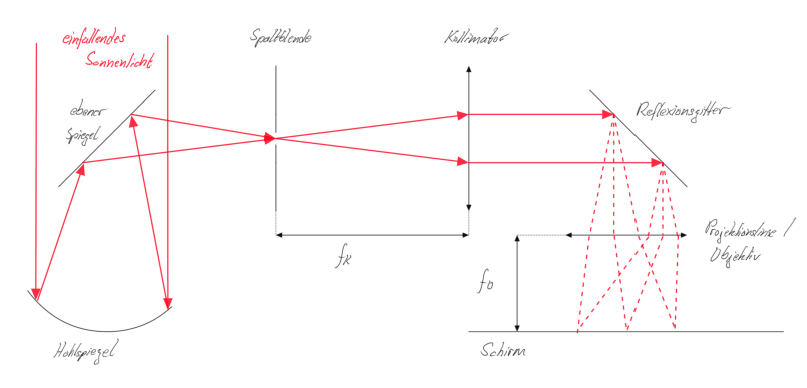
\includegraphics[scale=0.55]{skizzen/skizze-1.png}
			\caption{Skizze zum Aufbau des verwendeten Gitterspektrographen \\ $f_\mathrm{K}\ldots$Brennweite Kollimator \\ $f_\mathrm{O}\ldots$Brennweite Objektiv}
			\label{fig:skizze-spektrograph}
		\end{figure}

		Der grundsätzliche Aufbau des im Versuch verwendeten Gitterspektrographen ist in Abbildung \ref{fig:skizze-spektrograph} gezeigt.
		Hierbei wird das Sonnenlicht durch einen Hohlspiegel gebündelt und  durch eine Spaltblende zum Kollimator weitergeleitet.
		Durch den Spalt werden die Anteile des Lichts herausgefiltert, die nicht parallel zum Hohlspiegel eingefallen sind.
		Im Anschluss wird nun dieses divergierende Strahlenbündel mithilfe des Kollimators in ein rein paralleles Lichtbündel umgewandelt.
		Dieses trifft dann auf das Reflexionsgitter, welches wie ein typisches Gitter wirkt.
		Das Licht wird mit sich selbst interferieren, wodurch Beugungsmuster entstehen.
		Für große Entfernungen des Schirm interferieren näherungsweise parallele Strahlen miteinander.
		Die auftretenden Phänomene sind damit vergleichsweise leicht durch die Fraunhofer-Beugung berechenbar.
		Der Aufbau befindet sich jedoch in einem relativ kleinen geschlossenen System.
		Um die Bedingung, dass parallele Strahlen interferieren, dennoch nicht zu verletzen, werden durch eine Projektionslinse (auch Objektiv) parallel verlaufende Strahlen in einem Punkt auf dem Schirm fokussiert.
		Der Schirm zeigt also gerade die Spektrallinien des einfallendes Lichtes.

		Für den Abstand $x(n,\lambda)$ von der nullten Ordnung der Spektrallinie $n$.Ordnung mit Wellenlänge $\lambda$ ergibt sich dann näherungsweise
		\[ x(n,\lambda) = \frac{s}{g}n\lambda \]
		Dabei beschreibt $s$ den Abstand vom Gitter zum Schirm und $g$ die Gitterkonstante.
		Für das Auflösungsvermögen folgt dann
		\[ \frac{\lambda}{\Delta\lambda(n)} = \frac{x(n,\lambda)}{\Delta x(n,\lambda)} = nN \]
		wenn $N$ die Anzahl der beleuchteten Spalte am Reflexionsgitter beschreibt.

		Alle Berechnungen beruhen darauf, dass es sich um einen idealen Spektrographen handelt.
		Das heißt vor Allem, dass dabei die Spaltbreite der Spaltblende als gegen Null tendierend angenommen wird.
		Dies kann im Allgemeinen allerdings nicht realisiert werden, da sonst die Lichtintensität zu klein wäre.
		Aus diesem Grund wird das eigentliche Auflösungsvermögen stark durch die Spaltbreite bestimmt.
		Jede Spektrallinie ist dann eine Abbildung des Spalts.
	
	% subsection gitterspektrograph (end)

	\subsection{CCD-Detektor} % (fold)
	\label{sub:ccd_detektor}

		Um die Spektrallinien am Spektrograph messen zu können, wird der in Abbildung \ref{fig:skizze-spektrograph} beschriebene Schirm durch einen CCD-Detektor ersetzt.
		CCD-Detektoren bestehen aus einer Matrix lichtempfindlicher Fotodioden.
		Eine einfache Darstellung ist in Abbildung \ref{fig:schema-ccd} sichtbar.
		Einfallendes Licht überträgt durch den inneren photoelektrischen Effekt seine Energie auf die Elektronen der Halbleiter. 
		Dabei entstehen gleichzeitig negativ geladene freie Elektronen und positiv geladene \glqq Löcher\grqq, die sich aufgrund einer angelegten Spannung voneinander trennen. 
		Die Ladungen fließen jedoch nicht wie bei einer normalen Fotodiode sofort nach außen ab, sondern werden in der Speicherzelle selbst, in einem sogenannten Potentialtopf gesammelt, der wie ein Kondensator Ladungen speichert. 
		Die Ladungsmenge ist dabei proportional zur eingestrahlten Lichtmenge, wenn rechtzeitig ausgelesen wird, bevor die Leerlaufspannung der Fotodiode erreicht ist.
		Nach der Belichtung werden die Ladungen schrittweise verschoben, bis sie schließlich als Ladungspakete, eines nach dem anderen, den Ausleseverstärker erreichen. 
		Es wird eine von der Ladung und somit der Lichtmenge abhängige elektrische Spannung ausgegeben.
		Das Ausgangssignal des Sensors ist somit seriell.
		Durch Anwendung dieser Technik reicht es, bei der technischen Herstellung des CCD-Sensors einen Ausleseverstärker für die gesamte Matrix von Fotodioden zu verwenden.

		\begin{figure}
			\center
			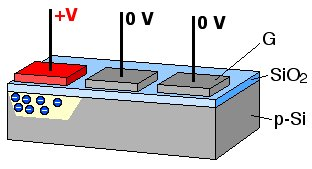
\includegraphics[scale=0.8]{referenzen/CCD_charge_transfer_animation.jpg}
			\caption{Schema eines CCD-Sensors (Quelle:\\ https://de.wikipedia.org/wiki/CCD-Sensor\#/media/File:CCD\_charge\_transfer\_animation.gif)}
			\label{fig:schema-ccd}
		\end{figure}

		Fotodioden eines CCD-Sensors können rechteckig, quadratisch oder polygonal sein, mit Kantenlängen von $1.4\unit{$\mu$m}$ bis über $20\unit{$\mu$m}$.
		Je größer die Fläche der Pixel, desto höher sind die Lichtempfindlichkeit und der Dynamikumfang, desto kleiner ist aber, bei gleicher Sensorgröße, die Bildauflösung.
		Bei Überbelichtung können Ladungen aus dem Potentialtopf einer Zelle in die Nachbarzellen übertreten.
		Die Messung von hohen Lichtintensitäten ist damit begrenzt.
		Abhilfe schaffte während des Versuches ein Papierfilter und die Einstellung einer kürzeren Belichtungszeit.

		Um nun mit dem CCD-Detektor auch Abstände oder Positionen messen zu können, muss ein bereits bekanntes Spektrum aufgenommen werden.
		So lassen sich dann mithilfe charakteristischer Spektrallinien die Skalierung $\alpha$ (Wellenlängenzunahme pro Pixel) und das Offset $\beta$ (Wellenlänge des linken äußersten Pixel) bestimmen.
		Näherungsweise können alle Funktionen als linear angesehen werden.
		Seien nun für zwei Wellenlängen $\lambda_1, \lambda_2$ mit $\lambda_1 < \lambda_2$ die Position bzw. die Pixel $p_1,p_2$ der Spektrallinien gegeben.
		Dann ergibt sich
		\begin{alignat*}{3}
			\alpha &= \frac{\lambda_2 - \lambda_1}{p_2 - p_1} \\
			\beta &= \lambda_1 - \alpha p_1
		\end{alignat*}
		Für die Wellenlänge eines beliebigen Pixels folgt dann, wenn alle Einstellungen am CCD-Detektor und am Spektrographen konstant bleiben
		\[ \lambda(p) = \alpha p + \beta \]
		Für gewisse Einstellungen und untersuchte Bereiche könnte diese Näherung verletzt werden.
		Um dies zu untersuchen, werden die gerade angegebenen Kalibrierungen nicht nur mit zwei Spektrallinien, sondern mit Mehreren an verschiedenen Stellen durchgeführt.

		Zur Auswertung der Intensitäten von Spektrallinien oder anderen Peaks ist es notwendig systematische und zufällige Fehler des CCD-Detektors zu kennen oder zu bestimmen.
		Hierfür spielen vor Allem die Kenngrößen Biaslevel, Rauschen und Dunkelstrom eine wichtige Rolle.
		
		Um ein Spannungssignal für verschiedene Pixel vom CCD-Sensor zu erhalten, werden, die Ladungen seriell ausgelesen, indem man die Ladungen von Diode zu Diode verschiebt.
		Bei dieser Verschiebung entsteht ein systematischer Fehler und eine statistische Abweichung (auch Rauschen) für jeden Pixel.
		Nach Beendigung des Auslesevorgangs wird zu jedem erhaltenen Wert ein sogenanntes Offset hinzuaddiert.
		Das Biaslevel eines Pixels ist dann gerade dieses Offset plus der systematische Fehler.

		Treffen keine Photonen auf den CCD-Sensor, so werden dennoch in jeder Fotodiode weitere Elektronen freigesetzt.
		Dieser Effekt entsteht durch die temperaturbedingte Bewegung der Elektronen, welche durch die geringe Bandlücke im Halbleiter ausreicht die Potentialbarriere zu überwinden.
		Die Anzahl der Elektronen pro Zeiteinheit, die so entstehen, wird Dunkelstrom genannt.
		Er ist jedoch unabhängig vom Photoneneinfall bzw. der Lichtintensität und somit ein Fehler in der Aufnahme.

	% subsection ccd_detektor (end)

	\subsection{Sonnenspektrum} % (fold)
	\label{sub:sonnenspektrum}

		Das elektromagnetische Spektrum der Sonne hat die größte Intensität im Bereich des sichtbaren Lichts. 
		Abhängig von der Wellenlänge wird die Sonnenstrahlung von der Atmosphäre mehr oder weniger stark absorbiert. 
		Die an der Erdoberfläche eintreffende Intensität hängt zudem stark vom Wetter und vom Sonnenstand ab.
		Beispiele des Sonnenspektrums zeigen die im Anhang \ref{sec:beispiele_des_sonnenspektrums} sichtbaren Abbildungen \ref{fig:sonnenspektrum-1} und \ref{fig:sonnenspektrum-2}.
		Das Spektrum ist von etwa $140 \unit{nm}$ bis etwa $10 \unit{cm}$ näherungsweise das eines Schwarzen Strahlers bei einer Temperatur von knapp $6000 \unit{K}$, der Temperatur der Photosphäre.
		Im Bereich von naher Infrarotstrahlung bis ins UV enthält das Spektrum eine Vielzahl von Absorptionslinien, die sogenannten Fraunhoferlinien. 
		Sie entstehen durch Strahlungsabsorption in der Chromosphäre der Sonne.
	
	% subsection sonnenspektrum (end)

% section grundlagen (end)
	\FloatBarrier
	\null
	\newpage
	\section{Versuchsaufbau und Durchführung} % (fold)
\label{sec:versuchsaufbau_und_durchf_hrung}

	\subsection{Aufbau des Michelson-Interferometers} % (fold)
	\label{sub:aufbau_des_michelson_interferometers}

	\begin{figure}[htb]
		\centering
		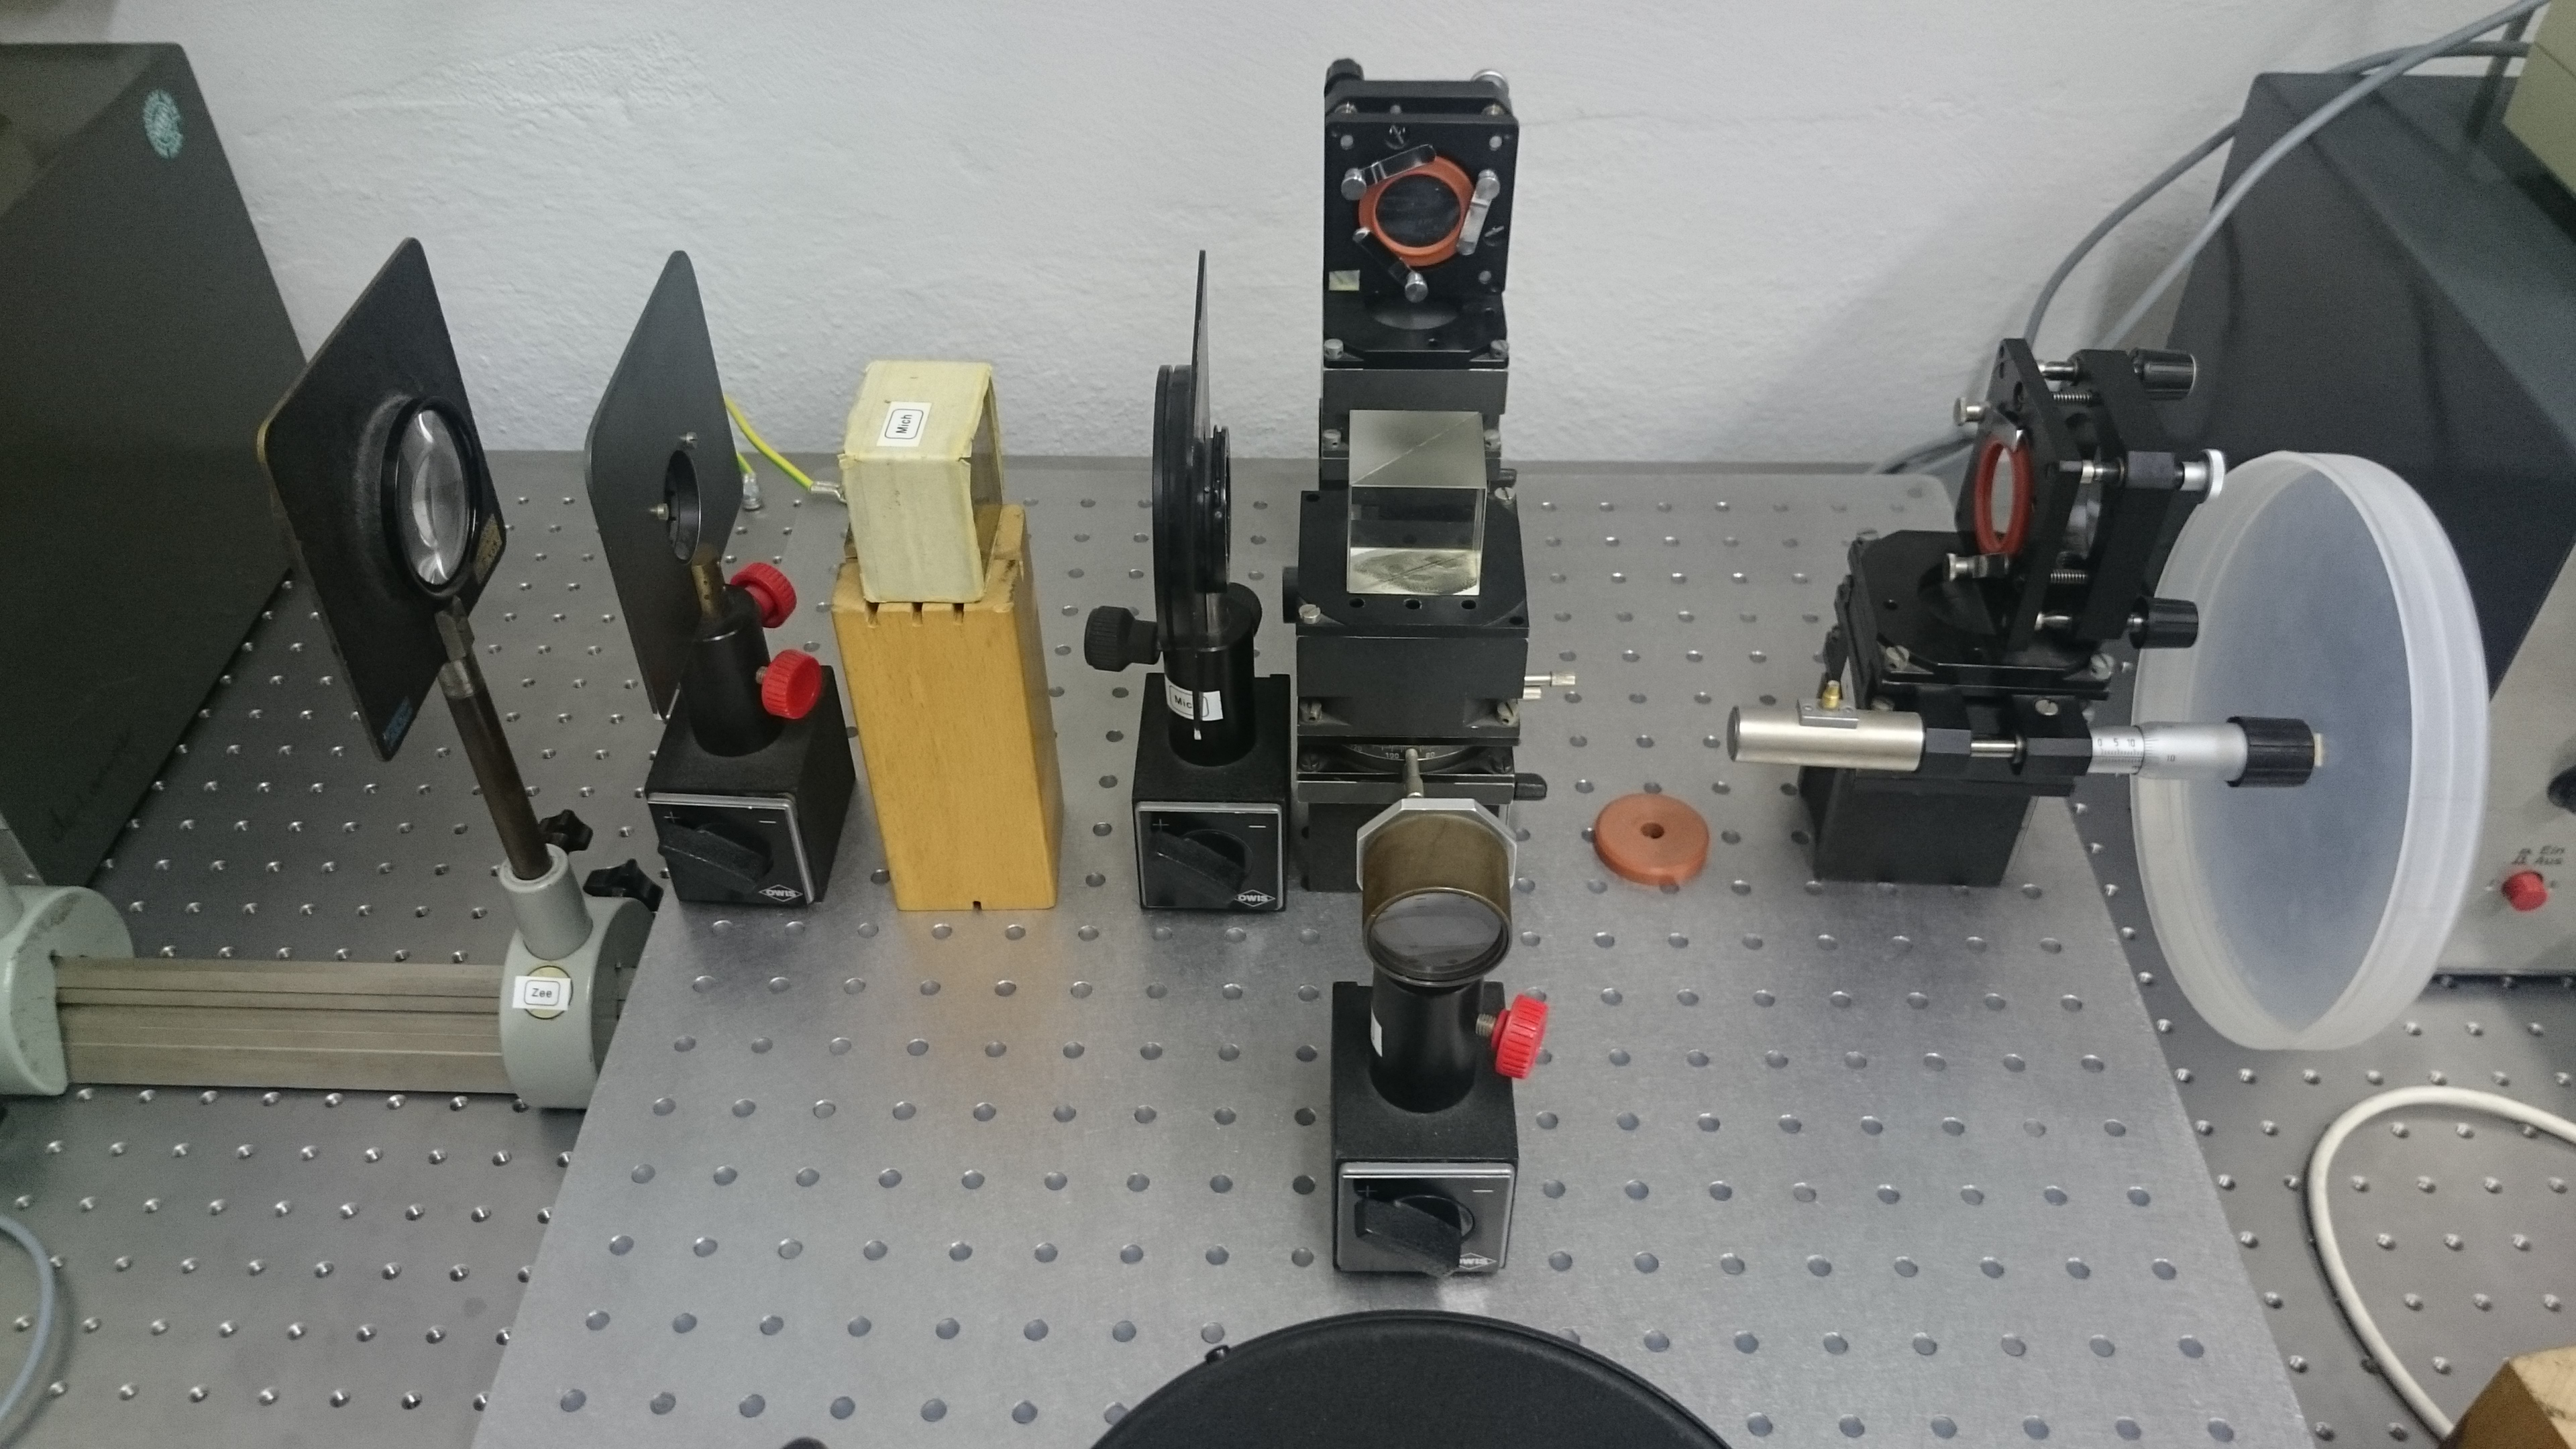
\includegraphics[scale = 0.08]{images/DSC_1011.JPG}
		\caption{Montagetisch mit Versuchsaufbau des MIF}
		\label{fig:aufbau-mif-1}
	\end{figure}

	In Abbildung \ref{fig:aufbau-mif-1} ist der Aufbau des MIF zu sehen, wie er unter Abschnitt \ref{sub:prinzip_des_michelson_interferometers} beschrieben wurde.
	Als Lichtquelle können eine Hg-Dampflampe mit verschiedenene Filtern sowie eine herkömmliche Glühlampe verwendet werden.
	Spiegel 2 ist über eine Mikrometerschraube in x-Richtung zu verstellen, drei weitere Feingewindeschrauben sind für die Winkeleinstellung vorgesehen.
	Durch Verwendung des Strahlteilerwürfels entfällt die sonst notwendige Kompensationsplatte.
	Neben der direkten Möglichkeit zur Beobachtung durch Blicken in den Strahlteiler, kann der Strahl auch noch mittels einer weiteren Linse und eines Ablenkspiegels auf Papier abgebildet und abfotografiert werden.
	
	% subsection aufbau_des_michelson_interferometers (end)


	\subsection{Aufbau des Fourier-Spektrometers} % (fold)
	\label{sub:aufabu_des_fourier_spektrometers}
	

	\begin{figure}[htb]
		\centering
		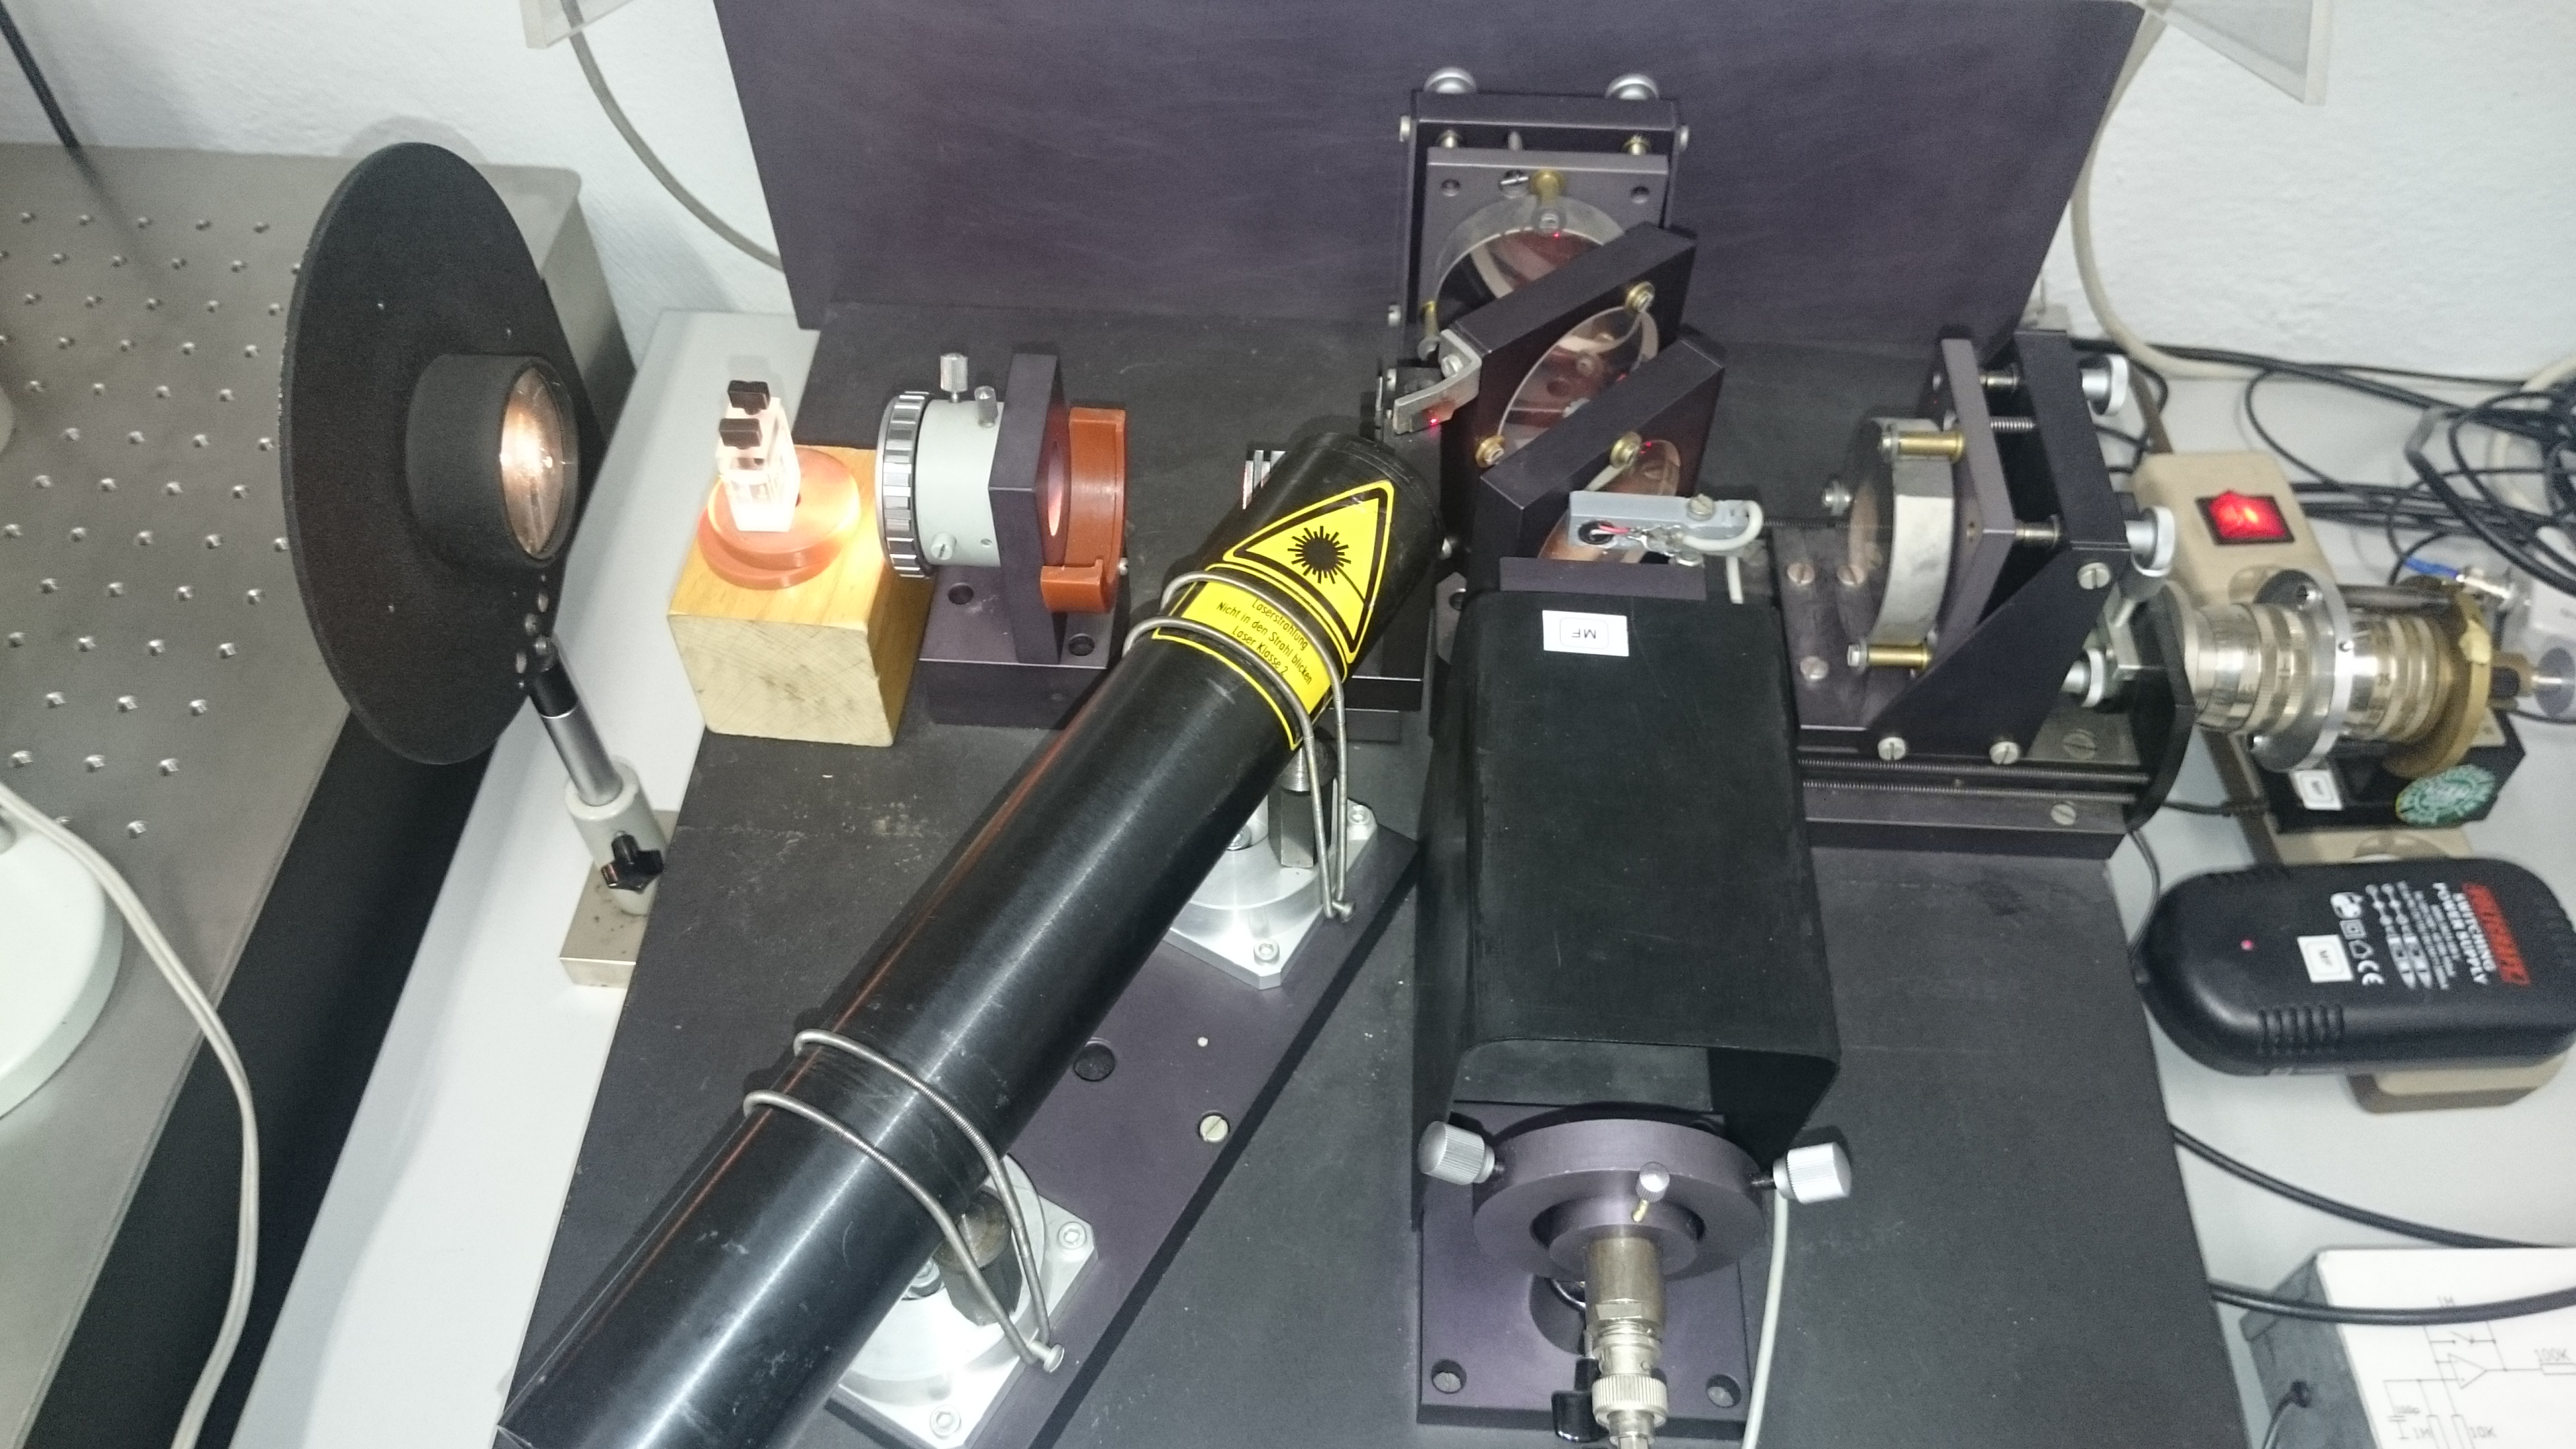
\includegraphics[scale = 0.08]{images/DSC_1010.JPG}
		\caption{Komponenten des Fourier-Spektrometers mit geöffneter Abdeckklappe}
		\label{fig:aufbau-mif-2}
	\end{figure}

	Abbildung \ref{fig:aufbau-mif-2} zeigt alle Komponeneten des Fourierspektrometers wie es im Versuch verwendet wurde.
	Links befindet sich die Lichtquelle.
	Als solche werden im Versuch Hg-Lampe, Na-Lampe, grüne LED, rote Laser-LED, Gas-Laser und Glühlampe verwendet.
	Zwischen Lampe und Kollimator können Filter oder Proben zur Absorbtion platziert werden.
	In der Mitte teilt ein halbdurchlässiger Spiegel den Strahl, kurz darüber ist die Kompensationsplatte zu finden.
	Spiegel 2 kann mittels einer Mikrometerschraube und den dahinter befindlichen Motor über den Computer gesteuert werden.
	Unter dem Strahlteiler befindet sich eine Linse, die den Strahl auf den Detektor bündelt.
	Auf der Linse befindet sich der Detektor für das Laser-Referenzsignal.
	An diesem wird die Messung anschließend angepasst und kalibriert.
	Akkumulierung der Datenpunkte, Aufzeichnen des Interferogramms und Erstellen der zugehörigen FFT (Fast Fourier Transformation) werden von einem LabView-Programm erledigt.
	Es dient ebenfalls zum Ansteuern des Motors von Spiegel 2.

	% subsection aufabu_des_fourier_spektrometers (end)


% section versuchsaufbau_und_durchf_hrung (end)
	\FloatBarrier
	\null
	\newpage
	\section{Messwerte und Auswertung} % (fold)
\label{sec:messwerte_und_auswertung}

	\subsection{Michelson-Interferometrie} % (fold)
	\label{sub:michelson_interferometrie}
	
		\subsubsection{Fizeau-Streifen und Haidinger Ringe} % (fold)
		\label{ssub:fizeau_streifen}

			Die Interferenzen gleicher Dicke wurden durch Verkippen von Spiegel 2 erzeugt.
			Dabei entstanden die horizontalen Streifen aus Abbildung \ref{fig:fizeau-h-1} durch Drehung um die horizontale $y$-Achse senkrecht zur Verschiebungsrichtung $x$.
			Analog ließen sich die vertikalen Interferenzmuster durch Drehung um die Vertikale, also die z-Achse bilden.
			Während man bei den senkrechten Interferenzmuster von Abbildung \ref{fig:fizeau-v} gerade Steifen erkennt, die zur Seite jedoch einen größeren Abstand aufweisen, sieht man die Streifen von Abbildung \ref{fig:fizeau-h-1} in annähernd gleichem Abstand, jedoch verzerrt.
			Beides spricht in diesem Fall für eine Spiegelkrümmung einer der beiden Spiegel in $z$-Richtung.
		
			\begin{figure}[htb]
				\begin{subfigure}[b]{.45\textwidth}
					\centering
					\includegraphics[scale=0.07]{messwerte/fizeau-streifen-h-1.png}
					\caption{Drehung um $y$-Achse}
					\label{fig:fizeau-h-1}
				\end{subfigure}
				\begin{subfigure}[b]{.55\textwidth}
					\centering
					\includegraphics[scale=0.0775]{messwerte/fizeau-streifen-v-1.png}
					\caption{Drehung um $z$-Achse}
					\label{fig:fizeau-v}
				\end{subfigure}
				\caption{Fizeau-Streifen durch Interferenz der grünen Hg-Dampflinie bei $\lambda = 546 \unit{nm}$}
			\end{figure}

			Mit Hilfe des Maxima-Abstandes und der unter \ref{sub:interferenzen_gleicher_dicke_fizeau_streifen} angegebenen Formel, kann man in etwa den Winkel der Verkippung ausrechnen.
			Um die Abstände zu normieren wird angenommen, dass das Bild nur durch die letzte Linse vergrößert wird und somit der ursprüngliche Durchmesser des Bildes gleich dem Linsendurchmesser ist, welcher im Versuch zu $D = 3 \unit{cm} $ bestimmt wurde.
			Im Durchschnitt beträgt der Streifenabstand der senkrechten Streifen dann in etwa $a = 0.75 \unit{cm}$.
			\[ \implies \quad \sin(\alpha /2) = \frac{\lambda}{2 a} = \frac{546 \unit{nm}}{2 \cdot 0.75 \unit{cm}} 
			\approx 3.64 \cdot 10^{-5} \]
			\[ \implies \quad \alpha \approx 7.3 \cdot 10^{-5} = 15\,^{\prime\prime} \]
			Betrachtet man den zweit untersten horizontalen Streifen in Abbildung \ref{fig:fizeau-h-1} dann beträgt die Höhendifferenz zwischen Mitte und Rand in etwa die gesamte Breite des Maximums.
			Folglich wird die Abweichung von der planen Fläche eines der beiden Spiegel auch in dem Bereich von $\lambda$ also etwa $0.5\,\mu\mathrm{m}$ liegen.

			Die Haidinger-Ringe konnten mit etwas Feingefühl zwar eingestellt werden und zeigten auch das unter \ref{sub:interferenzen_gleicher_neigung_haidinger_ringe} gezeigte Verhalten, ließen sich allerdings aufgrund des schwachen Kontrastes und der geringen Leuchtstärke im Vergleich zu anderen Reflexen nicht durch die Kamera aufnehmen.


		% subsubsection fizeau_streifen (end)

		\subsubsection{Einlfuss der Glasplatte} % (fold)
		\label{ssub:einlfuss_der_glasplatte}

			Das MIF findet auch Anwendung bei der Bewertung der Güte optischer Bauteile.
			Als Beispiel wurde hier der Einfluss einer scheinbar planparallelen Glasplatte auf die Interferenzmuster untersucht.
			Dazu stellten wir zunächst eine möglichst geringe Spiegelverschiebung ein, also den Bereich der Haidinger-Ringe, zu erahnen in Abbildung \ref{fig:ohne_platte}.
			Als nächstes wurde die Platte in Strahlengang 2 gestellt.
			Wie man in Bild \ref{fig:mit_platte} sehen kann tauchen nun Fizeau-Streifen auf, was bedeutet, dass die Platte einen ähnlichen Einfluss wie die Spiegelverkippung hat.
			Daraus folgt, dass sie an einer Seite dicker sein muss als an der anderen und dadurch der optische Weg hier verlängert wird.
			In Aufnahme \ref{fig:mit_platte} ist zu erkennen, dass der Unterschied auf den Diagonalen am größten sein muss.
			Das Erscheinen von 5 Streifen bedeutet eine maximale Wegdifferenz von $5 \lambda$.
			Für die Glasplatte mit einem Brechnungsindex von $n_\m{Glas}=1.5$ bedeutet das eine Stärkendifferenz von:
			\[ \Delta d = \frac{5 \lambda}{2 (n_\m{Glas} - n_\m{Luft}) } \approx 2.7\,\mu\m{m} \]

			\begin{figure}[htb]
				\begin{subfigure}[b]{.5\textwidth}
					\centering
					\includegraphics[scale=0.07]{messwerte/harded-fucked-in-budapest-1.png}
					\caption{Ohne Glasplatte}
					\label{fig:ohne_platte}
				\end{subfigure}
				\begin{subfigure}[b]{.5\textwidth}
					\centering
					\includegraphics[scale=0.069]{messwerte/harded-fucked-in-budapest-2-extended-unedited-directors-cut.png}
					\caption{Mit Glasplatte}
					\label{fig:mit_platte}
				\end{subfigure}
				\caption{Interferenzmuster am MIF bei minimaler Wegdifferenz bei verwendeter Wellenlänge $\lambda = 546\unit{nm}$}
			\end{figure}
		
		% subsubsection einlfuss_der_glasplatte (end)

		\subsubsection{Weißlichtinterferenz} % (fold)
		\label{ssub:wei_lichtinterferenz}

			Auch das Licht eines thermischen Strahlers kann am MIF zur Interferenz gebracht werden.
			In Abbildung \ref{fig:weiss} ist dies zu sehen.
			Die Anforderung hierbei ist den sehr kleinen Bereich der Kohärenzlänge $l_\m{koh}$ genau einzustellen.
			Durch Verkippen von Spiegel 2 konnten wir nun wie im Bild zu erkennen maximal 7 Fizeau-Streifen erzeugen, bis die Wegdifferenz $2 \Delta x > l_\m{koh}$ war.
			Wenn wir für weißes Licht eine mittlere Wellenlänge von etwa $\overline{\lambda} = 550 \unit{nm} $ einsetzen erhalten wir als Abschätzung für die Kohärenzlänge:
			\[ l_\m{koh} = 7 \overline{\lambda} \approx 3.8\,\mu\m{m} \]

			\begin{figure}[htb]
				\centering
				\includegraphics[scale=0.13]{messwerte/weiss-1.png}
				\caption{Interferenz einer Weißlichtquelle (Glühlampe) am MIF}
				\label{fig:weiss}
			\end{figure}

		% subsubsection wei_lichtinterferenz (end)


		\subsubsection{Inhomogener Brechungsindex durch Wärme} % (fold)
		\label{ssub:inhomogener_brechungsindex_durch_w_rme}
			
			Die Empfindlichkeit des MIF konnte im Versuch mit einem heißen Widerstand demonstriert werden.
			Der Widerstand wurde im Strahlengang vor Spiegel 2 positioniert und die Luft über ihm erwärmt.
			Daraus resultierte eine Verminderung des Brechungsindex, was zu einer Verkürzung der optischen Weglänge führt.
			In Abbildung \ref{fig:hot ohm a} ist das Interferenzmuster mit eingebrachten Widerstand zu sehen.

			\begin{figure}[htb]
				\centering
				\includegraphics[scale=0.11]{messwerte/hot-ohm-a.png}
				\caption{Interferenzstreifen der grünen Hg-Dampflinie bei $\lambda = 546 \unit{nm}$ mit Wärmequelle im Strahlengang}
				\label{fig:hot ohm a}
			\end{figure}

			Man sieht, dass die regelmäßigen Fizeau-Streifen im linken Bereich verzerrt sind.
			Hier ist der Strahl durch heißere Luft propagiert.
			Die maximale Verschiebung kann anhand der Abbildung auf etwa ein $\lambda$ geschätzt werden.
			Damit ergibt sich über den insgesamt etwa $2 \unit{cm}$ langen Widerstand eine Weglängendifferenz von:
			\[ \lambda = 2\cdot 2 \unit{cm} \cdot (n_\m{cold} - n_\m{hot}) \]
			\[ \implies \quad \Delta n \approx 1.4\cdot 10^{-5} \]

		% subsubsection inhomogener_brechungsindex_durch_w_rme (end)

	% subsection michelson_interferometrie (end)

	\subsection{Fourier-Spektroskopie} % (fold)
	\label{sub:fourier_spektroskopie}

		\subsubsection{Parameter und Auflösevermögen} % (fold)
		\label{ssub:parameter_und_aufl_severm_gen}

			Zum Verdeutlichen des Prinzips, des Fourier-Spektrometers (FS) wurden zunächst zwei Schwingungen am Frequenzgenerator erzeugt und überlagert.
			Diese besaßen eine geringe Frequenzdifferenz $\Delta f$, um somit eine Schwebung zu erzeugen.
			Die FFT des Interferogramms ist in den Abbildungen \ref{fig:schwebung-1} und \ref{fig:schwebung-2} für verschiedene Aufnahmeparameter zu sehen.
			Es ist natürlich zu beachten, dass die unten angegebene Wellenlänge hier nicht der wirklichen Wellenlänge der Signale entspricht, was aber für das Auflösevermögen keine Rolle spielt.
			Wie man klar erkennen kann, können die beiden Frequenzen im ersten Bild aufgelöst werden, währenddessen sich im zweiten Bild aufgrund der geringen Sampleanzahl die Auflösung verschlechtert und somit die einzelnen Peaks nicht mehr getrennt werden können.
			Mit der Gleichung welche in Grundlagen unter Abschnitt \ref{sub:fourierspektroskopie} angegeben ist, lässt sich nun das Auflösungsvermögen für beide Aufnahmen berechnen.
			Zu beachten ist hier die Annahme, dass der Motor die konstante Geschwindigkeit $v = 10\,\mu\m{m}s^{-1}$ hält.
			Die jeweilige Aufnahmezeiten $T$ beträgt jeweils $S/sps$ und die Wellenlängen liegen im Bereich um $504 \unit{nm}$.
			\[ \curvb{\frac{\lambda}{\Delta \lambda}}_1 = \frac{2 v T_1}{\lambda} \approx 3900,\qquad \curvb{\frac{\lambda}{\Delta \lambda}}_2 = \frac{2 v T_2}{\lambda} \approx 39 \]
			Für das minimal benötigte Auflösungsvermögen gilt:
			\[ \curvb{\frac{\lambda}{\Delta \lambda}}_\m{min} = \frac{504 \unit{nm}}{2 \unit{nm}} \approx 250 \]

			\begin{figure}[htb]
				\centering
				% GNUPLOT: LaTeX picture with Postscript
\begingroup
  \makeatletter
  \providecommand\color[2][]{%
    \GenericError{(gnuplot) \space\space\space\@spaces}{%
      Package color not loaded in conjunction with
      terminal option `colourtext'%
    }{See the gnuplot documentation for explanation.%
    }{Either use 'blacktext' in gnuplot or load the package
      color.sty in LaTeX.}%
    \renewcommand\color[2][]{}%
  }%
  \providecommand\includegraphics[2][]{%
    \GenericError{(gnuplot) \space\space\space\@spaces}{%
      Package graphicx or graphics not loaded%
    }{See the gnuplot documentation for explanation.%
    }{The gnuplot epslatex terminal needs graphicx.sty or graphics.sty.}%
    \renewcommand\includegraphics[2][]{}%
  }%
  \providecommand\rotatebox[2]{#2}%
  \@ifundefined{ifGPcolor}{%
    \newif\ifGPcolor
    \GPcolorfalse
  }{}%
  \@ifundefined{ifGPblacktext}{%
    \newif\ifGPblacktext
    \GPblacktexttrue
  }{}%
  % define a \g@addto@macro without @ in the name:
  \let\gplgaddtomacro\g@addto@macro
  % define empty templates for all commands taking text:
  \gdef\gplbacktext{}%
  \gdef\gplfronttext{}%
  \makeatother
  \ifGPblacktext
    % no textcolor at all
    \def\colorrgb#1{}%
    \def\colorgray#1{}%
  \else
    % gray or color?
    \ifGPcolor
      \def\colorrgb#1{\color[rgb]{#1}}%
      \def\colorgray#1{\color[gray]{#1}}%
      \expandafter\def\csname LTw\endcsname{\color{white}}%
      \expandafter\def\csname LTb\endcsname{\color{black}}%
      \expandafter\def\csname LTa\endcsname{\color{black}}%
      \expandafter\def\csname LT0\endcsname{\color[rgb]{1,0,0}}%
      \expandafter\def\csname LT1\endcsname{\color[rgb]{0,1,0}}%
      \expandafter\def\csname LT2\endcsname{\color[rgb]{0,0,1}}%
      \expandafter\def\csname LT3\endcsname{\color[rgb]{1,0,1}}%
      \expandafter\def\csname LT4\endcsname{\color[rgb]{0,1,1}}%
      \expandafter\def\csname LT5\endcsname{\color[rgb]{1,1,0}}%
      \expandafter\def\csname LT6\endcsname{\color[rgb]{0,0,0}}%
      \expandafter\def\csname LT7\endcsname{\color[rgb]{1,0.3,0}}%
      \expandafter\def\csname LT8\endcsname{\color[rgb]{0.5,0.5,0.5}}%
    \else
      % gray
      \def\colorrgb#1{\color{black}}%
      \def\colorgray#1{\color[gray]{#1}}%
      \expandafter\def\csname LTw\endcsname{\color{white}}%
      \expandafter\def\csname LTb\endcsname{\color{black}}%
      \expandafter\def\csname LTa\endcsname{\color{black}}%
      \expandafter\def\csname LT0\endcsname{\color{black}}%
      \expandafter\def\csname LT1\endcsname{\color{black}}%
      \expandafter\def\csname LT2\endcsname{\color{black}}%
      \expandafter\def\csname LT3\endcsname{\color{black}}%
      \expandafter\def\csname LT4\endcsname{\color{black}}%
      \expandafter\def\csname LT5\endcsname{\color{black}}%
      \expandafter\def\csname LT6\endcsname{\color{black}}%
      \expandafter\def\csname LT7\endcsname{\color{black}}%
      \expandafter\def\csname LT8\endcsname{\color{black}}%
    \fi
  \fi
  \setlength{\unitlength}{0.0500bp}%
  \begin{picture}(6802.00,3968.00)%
    \gplgaddtomacro\gplbacktext{%
      \csname LTb\endcsname%
      \put(946,954){\makebox(0,0)[r]{\strut{} 0}}%
      \put(946,1454){\makebox(0,0)[r]{\strut{} 0.2}}%
      \put(946,1954){\makebox(0,0)[r]{\strut{} 0.4}}%
      \put(946,2453){\makebox(0,0)[r]{\strut{} 0.6}}%
      \put(946,2953){\makebox(0,0)[r]{\strut{} 0.8}}%
      \put(946,3453){\makebox(0,0)[r]{\strut{} 1}}%
      \put(1522,484){\makebox(0,0){\strut{} 496}}%
      \put(2410,484){\makebox(0,0){\strut{} 498}}%
      \put(3298,484){\makebox(0,0){\strut{} 500}}%
      \put(4185,484){\makebox(0,0){\strut{} 502}}%
      \put(5073,484){\makebox(0,0){\strut{} 504}}%
      \put(5961,484){\makebox(0,0){\strut{} 506}}%
      \put(176,2203){\rotatebox{-270}{\makebox(0,0){\strut{}Intensität}}}%
      \put(3741,154){\makebox(0,0){\strut{}Wellenlänge $\lambda \ [\unit{nm}]$}}%
    }%
    \gplgaddtomacro\gplfronttext{%
      \csname LTb\endcsname%
      \put(2398,3530){\makebox(0,0)[r]{\strut{}Messwerte}}%
    }%
    \gplbacktext
    \put(0,0){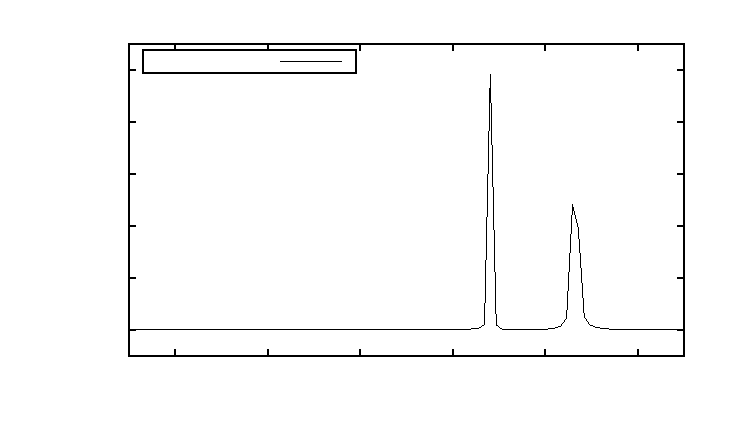
\includegraphics{schwebung-1}}%
    \gplfronttext
  \end{picture}%
\endgroup

				\caption{FFT des Interferogramms der überlagerten Sinusschwingungen mit $1000\unit{sps}$ und $100000$ Samples}
				\label{fig:schwebung-1}
			\end{figure}

			\begin{figure}[htb]
				\centering
				% GNUPLOT: LaTeX picture with Postscript
\begingroup
  \makeatletter
  \providecommand\color[2][]{%
    \GenericError{(gnuplot) \space\space\space\@spaces}{%
      Package color not loaded in conjunction with
      terminal option `colourtext'%
    }{See the gnuplot documentation for explanation.%
    }{Either use 'blacktext' in gnuplot or load the package
      color.sty in LaTeX.}%
    \renewcommand\color[2][]{}%
  }%
  \providecommand\includegraphics[2][]{%
    \GenericError{(gnuplot) \space\space\space\@spaces}{%
      Package graphicx or graphics not loaded%
    }{See the gnuplot documentation for explanation.%
    }{The gnuplot epslatex terminal needs graphicx.sty or graphics.sty.}%
    \renewcommand\includegraphics[2][]{}%
  }%
  \providecommand\rotatebox[2]{#2}%
  \@ifundefined{ifGPcolor}{%
    \newif\ifGPcolor
    \GPcolorfalse
  }{}%
  \@ifundefined{ifGPblacktext}{%
    \newif\ifGPblacktext
    \GPblacktexttrue
  }{}%
  % define a \g@addto@macro without @ in the name:
  \let\gplgaddtomacro\g@addto@macro
  % define empty templates for all commands taking text:
  \gdef\gplbacktext{}%
  \gdef\gplfronttext{}%
  \makeatother
  \ifGPblacktext
    % no textcolor at all
    \def\colorrgb#1{}%
    \def\colorgray#1{}%
  \else
    % gray or color?
    \ifGPcolor
      \def\colorrgb#1{\color[rgb]{#1}}%
      \def\colorgray#1{\color[gray]{#1}}%
      \expandafter\def\csname LTw\endcsname{\color{white}}%
      \expandafter\def\csname LTb\endcsname{\color{black}}%
      \expandafter\def\csname LTa\endcsname{\color{black}}%
      \expandafter\def\csname LT0\endcsname{\color[rgb]{1,0,0}}%
      \expandafter\def\csname LT1\endcsname{\color[rgb]{0,1,0}}%
      \expandafter\def\csname LT2\endcsname{\color[rgb]{0,0,1}}%
      \expandafter\def\csname LT3\endcsname{\color[rgb]{1,0,1}}%
      \expandafter\def\csname LT4\endcsname{\color[rgb]{0,1,1}}%
      \expandafter\def\csname LT5\endcsname{\color[rgb]{1,1,0}}%
      \expandafter\def\csname LT6\endcsname{\color[rgb]{0,0,0}}%
      \expandafter\def\csname LT7\endcsname{\color[rgb]{1,0.3,0}}%
      \expandafter\def\csname LT8\endcsname{\color[rgb]{0.5,0.5,0.5}}%
    \else
      % gray
      \def\colorrgb#1{\color{black}}%
      \def\colorgray#1{\color[gray]{#1}}%
      \expandafter\def\csname LTw\endcsname{\color{white}}%
      \expandafter\def\csname LTb\endcsname{\color{black}}%
      \expandafter\def\csname LTa\endcsname{\color{black}}%
      \expandafter\def\csname LT0\endcsname{\color{black}}%
      \expandafter\def\csname LT1\endcsname{\color{black}}%
      \expandafter\def\csname LT2\endcsname{\color{black}}%
      \expandafter\def\csname LT3\endcsname{\color{black}}%
      \expandafter\def\csname LT4\endcsname{\color{black}}%
      \expandafter\def\csname LT5\endcsname{\color{black}}%
      \expandafter\def\csname LT6\endcsname{\color{black}}%
      \expandafter\def\csname LT7\endcsname{\color{black}}%
      \expandafter\def\csname LT8\endcsname{\color{black}}%
    \fi
  \fi
  \setlength{\unitlength}{0.0500bp}%
  \begin{picture}(6802.00,3968.00)%
    \gplgaddtomacro\gplbacktext{%
      \csname LTb\endcsname%
      \put(946,954){\makebox(0,0)[r]{\strut{} 0}}%
      \put(946,1454){\makebox(0,0)[r]{\strut{} 0.2}}%
      \put(946,1954){\makebox(0,0)[r]{\strut{} 0.4}}%
      \put(946,2453){\makebox(0,0)[r]{\strut{} 0.6}}%
      \put(946,2953){\makebox(0,0)[r]{\strut{} 0.8}}%
      \put(946,3453){\makebox(0,0)[r]{\strut{} 1}}%
      \put(1562,484){\makebox(0,0){\strut{} 460}}%
      \put(2531,484){\makebox(0,0){\strut{} 480}}%
      \put(3499,484){\makebox(0,0){\strut{} 500}}%
      \put(4468,484){\makebox(0,0){\strut{} 520}}%
      \put(5436,484){\makebox(0,0){\strut{} 540}}%
      \put(6405,484){\makebox(0,0){\strut{} 560}}%
      \put(176,2203){\rotatebox{-270}{\makebox(0,0){\strut{}Intensität}}}%
      \put(3741,154){\makebox(0,0){\strut{}Wellenlänge $\lambda \ [\unit{nm}]$}}%
    }%
    \gplgaddtomacro\gplfronttext{%
      \csname LTb\endcsname%
      \put(2398,3530){\makebox(0,0)[r]{\strut{}Messwerte}}%
    }%
    \gplbacktext
    \put(0,0){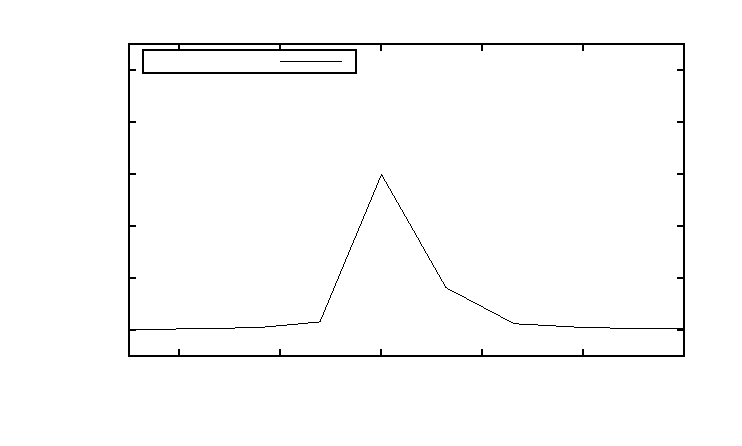
\includegraphics{schwebung-2}}%
    \gplfronttext
  \end{picture}%
\endgroup

				\caption{FFT des Interferogramms der überlagerten Sinusschwingungen mit $500\unit{sps}$ und $500$ Samples}
				\label{fig:schwebung-2}
			\end{figure}
 
		% subsubsection parameter_und_aufl_severm_gen (end)

		\subsubsection{Spektrum LED- und Gaslaser} % (fold)
		\label{ssub:spektrum_led_und_gaslaser}

			Im Folgenden wurden einige einfache Vergleichsspektren verschiedener LED- und Laserlichtquellen vermessen.
			In Abbildung \ref{fig:gr-led-spec} sieht man die Intensitätsverteilung einer grünen Leuchtdiode.
			Wie erwartet und liegt das Maximum der Intensitätsverteilung im Bereich von $550 \unit{nm}$, was im Auge einen grünen Farbeindruck erweckt.
			Die relativ Breite Verteilung des Spektrums von ca. $520 bis 600 \unit{nm}$ ist mit der Bandstruktur des Halbleitermaterials zu erklären.
			Das Maximum der Intensität wurde zu ungefähr $540 \unit{nm}$ bestimmt.
			Damit gilt für die Bandlücke:
			\[ \Delta E = \frac{hc}{\lambda} \approx 2.3 \unit{eV} \]

			Dagegen ist Spektrum einer Laser-LED in Graph \ref{fig:rot-laser-led} gezeigt.
			Durch die Resonatoren und die hohe Intensität im Bauteil setzen sich hier nur 2 Moden durch, wobei die erste bei 34567890 nm wesentlich stärker ausgeprägt ist, als die zweite im Abstand von 978 nm.

			Im dritten Bild sieht man nun noch das Spektrum eines frequenzverdoppelten Nd:Yag-Lasers.
			Dieser erzeugt zunächst Licht der Wellenlänge $1064 \unit{nm}$ (Quelle Bergmann und Schäfer Seite 882) welches anschließend durch den nichtlinearen Prozess der Frequenzverdopplung in einem Kristall zu großen Teilen zu Licht der halben Wellenlänge, also $532 \unit{nm}$ umgewandelt wird.
			Da der Detektor nur bis etwa $1000 \unit{nm}$ empfindlich ist (siehe Abschnitt \ref{ssub:gl_hlampenspektrum}) kann die ursprüngliche Frequenz hier nicht mehr dargestellt werden.
			Dafür sieht man überdeutlich den Peak bei ziemlich genau $532 \unit{nm}$ wie erwartet.
			Da für die Frequenzverdopplung spezielle Anforderungen für Frequenz und Wellenlänge im Kristall gelten, können sich hier auch andere Moden, selbst wenn sie im Nd:YAG-Laser entstehen würden nicht mehr effektiv verdoppeln, weshalb selbst bei hoher Auflösung (hier etwa 8000) nur ein Peak zu sehen ist. 

		
			\begin{figure}[htb]
				\centering
				% GNUPLOT: LaTeX picture with Postscript
\begingroup
  \makeatletter
  \providecommand\color[2][]{%
    \GenericError{(gnuplot) \space\space\space\@spaces}{%
      Package color not loaded in conjunction with
      terminal option `colourtext'%
    }{See the gnuplot documentation for explanation.%
    }{Either use 'blacktext' in gnuplot or load the package
      color.sty in LaTeX.}%
    \renewcommand\color[2][]{}%
  }%
  \providecommand\includegraphics[2][]{%
    \GenericError{(gnuplot) \space\space\space\@spaces}{%
      Package graphicx or graphics not loaded%
    }{See the gnuplot documentation for explanation.%
    }{The gnuplot epslatex terminal needs graphicx.sty or graphics.sty.}%
    \renewcommand\includegraphics[2][]{}%
  }%
  \providecommand\rotatebox[2]{#2}%
  \@ifundefined{ifGPcolor}{%
    \newif\ifGPcolor
    \GPcolorfalse
  }{}%
  \@ifundefined{ifGPblacktext}{%
    \newif\ifGPblacktext
    \GPblacktexttrue
  }{}%
  % define a \g@addto@macro without @ in the name:
  \let\gplgaddtomacro\g@addto@macro
  % define empty templates for all commands taking text:
  \gdef\gplbacktext{}%
  \gdef\gplfronttext{}%
  \makeatother
  \ifGPblacktext
    % no textcolor at all
    \def\colorrgb#1{}%
    \def\colorgray#1{}%
  \else
    % gray or color?
    \ifGPcolor
      \def\colorrgb#1{\color[rgb]{#1}}%
      \def\colorgray#1{\color[gray]{#1}}%
      \expandafter\def\csname LTw\endcsname{\color{white}}%
      \expandafter\def\csname LTb\endcsname{\color{black}}%
      \expandafter\def\csname LTa\endcsname{\color{black}}%
      \expandafter\def\csname LT0\endcsname{\color[rgb]{1,0,0}}%
      \expandafter\def\csname LT1\endcsname{\color[rgb]{0,1,0}}%
      \expandafter\def\csname LT2\endcsname{\color[rgb]{0,0,1}}%
      \expandafter\def\csname LT3\endcsname{\color[rgb]{1,0,1}}%
      \expandafter\def\csname LT4\endcsname{\color[rgb]{0,1,1}}%
      \expandafter\def\csname LT5\endcsname{\color[rgb]{1,1,0}}%
      \expandafter\def\csname LT6\endcsname{\color[rgb]{0,0,0}}%
      \expandafter\def\csname LT7\endcsname{\color[rgb]{1,0.3,0}}%
      \expandafter\def\csname LT8\endcsname{\color[rgb]{0.5,0.5,0.5}}%
    \else
      % gray
      \def\colorrgb#1{\color{black}}%
      \def\colorgray#1{\color[gray]{#1}}%
      \expandafter\def\csname LTw\endcsname{\color{white}}%
      \expandafter\def\csname LTb\endcsname{\color{black}}%
      \expandafter\def\csname LTa\endcsname{\color{black}}%
      \expandafter\def\csname LT0\endcsname{\color{black}}%
      \expandafter\def\csname LT1\endcsname{\color{black}}%
      \expandafter\def\csname LT2\endcsname{\color{black}}%
      \expandafter\def\csname LT3\endcsname{\color{black}}%
      \expandafter\def\csname LT4\endcsname{\color{black}}%
      \expandafter\def\csname LT5\endcsname{\color{black}}%
      \expandafter\def\csname LT6\endcsname{\color{black}}%
      \expandafter\def\csname LT7\endcsname{\color{black}}%
      \expandafter\def\csname LT8\endcsname{\color{black}}%
    \fi
  \fi
  \setlength{\unitlength}{0.0500bp}%
  \begin{picture}(6802.00,3968.00)%
    \gplgaddtomacro\gplbacktext{%
      \csname LTb\endcsname%
      \put(946,1004){\makebox(0,0)[r]{\strut{} 0}}%
      \put(946,1604){\makebox(0,0)[r]{\strut{} 0.2}}%
      \put(946,2204){\makebox(0,0)[r]{\strut{} 0.4}}%
      \put(946,2803){\makebox(0,0)[r]{\strut{} 0.6}}%
      \put(946,3403){\makebox(0,0)[r]{\strut{} 0.8}}%
      \put(1078,484){\makebox(0,0){\strut{} 450}}%
      \put(2410,484){\makebox(0,0){\strut{} 500}}%
      \put(3742,484){\makebox(0,0){\strut{} 550}}%
      \put(5073,484){\makebox(0,0){\strut{} 600}}%
      \put(6405,484){\makebox(0,0){\strut{} 650}}%
      \put(176,2203){\rotatebox{-270}{\makebox(0,0){\strut{}Intensität}}}%
      \put(3741,154){\makebox(0,0){\strut{}Wellenlänge $\lambda \ [\unit{nm}]$}}%
    }%
    \gplgaddtomacro\gplfronttext{%
      \csname LTb\endcsname%
      \put(2398,3530){\makebox(0,0)[r]{\strut{}Messwerte}}%
    }%
    \gplbacktext
    \put(0,0){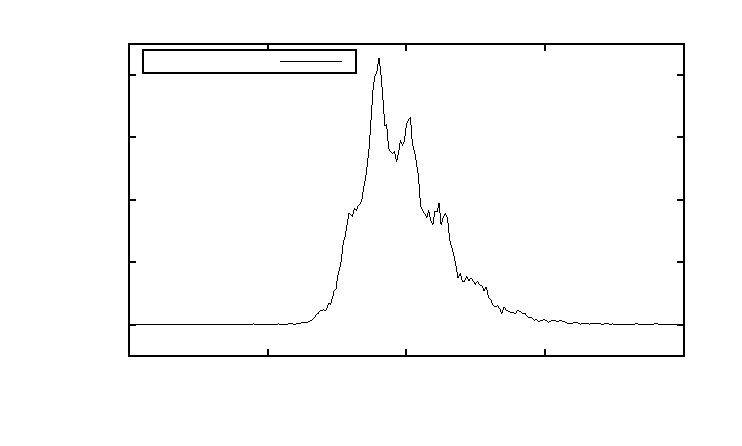
\includegraphics{led-spec}}%
    \gplfronttext
  \end{picture}%
\endgroup

				\caption{Spektrum einer grünen LED aufgenommen mit $10000$ Samples und $500 \unit{sps}$}
				\label{fig:gr-led-spec}
			\end{figure}

			\begin{figure}[htb]
				\centering
				% GNUPLOT: LaTeX picture with Postscript
\begingroup
  \makeatletter
  \providecommand\color[2][]{%
    \GenericError{(gnuplot) \space\space\space\@spaces}{%
      Package color not loaded in conjunction with
      terminal option `colourtext'%
    }{See the gnuplot documentation for explanation.%
    }{Either use 'blacktext' in gnuplot or load the package
      color.sty in LaTeX.}%
    \renewcommand\color[2][]{}%
  }%
  \providecommand\includegraphics[2][]{%
    \GenericError{(gnuplot) \space\space\space\@spaces}{%
      Package graphicx or graphics not loaded%
    }{See the gnuplot documentation for explanation.%
    }{The gnuplot epslatex terminal needs graphicx.sty or graphics.sty.}%
    \renewcommand\includegraphics[2][]{}%
  }%
  \providecommand\rotatebox[2]{#2}%
  \@ifundefined{ifGPcolor}{%
    \newif\ifGPcolor
    \GPcolorfalse
  }{}%
  \@ifundefined{ifGPblacktext}{%
    \newif\ifGPblacktext
    \GPblacktexttrue
  }{}%
  % define a \g@addto@macro without @ in the name:
  \let\gplgaddtomacro\g@addto@macro
  % define empty templates for all commands taking text:
  \gdef\gplbacktext{}%
  \gdef\gplfronttext{}%
  \makeatother
  \ifGPblacktext
    % no textcolor at all
    \def\colorrgb#1{}%
    \def\colorgray#1{}%
  \else
    % gray or color?
    \ifGPcolor
      \def\colorrgb#1{\color[rgb]{#1}}%
      \def\colorgray#1{\color[gray]{#1}}%
      \expandafter\def\csname LTw\endcsname{\color{white}}%
      \expandafter\def\csname LTb\endcsname{\color{black}}%
      \expandafter\def\csname LTa\endcsname{\color{black}}%
      \expandafter\def\csname LT0\endcsname{\color[rgb]{1,0,0}}%
      \expandafter\def\csname LT1\endcsname{\color[rgb]{0,1,0}}%
      \expandafter\def\csname LT2\endcsname{\color[rgb]{0,0,1}}%
      \expandafter\def\csname LT3\endcsname{\color[rgb]{1,0,1}}%
      \expandafter\def\csname LT4\endcsname{\color[rgb]{0,1,1}}%
      \expandafter\def\csname LT5\endcsname{\color[rgb]{1,1,0}}%
      \expandafter\def\csname LT6\endcsname{\color[rgb]{0,0,0}}%
      \expandafter\def\csname LT7\endcsname{\color[rgb]{1,0.3,0}}%
      \expandafter\def\csname LT8\endcsname{\color[rgb]{0.5,0.5,0.5}}%
    \else
      % gray
      \def\colorrgb#1{\color{black}}%
      \def\colorgray#1{\color[gray]{#1}}%
      \expandafter\def\csname LTw\endcsname{\color{white}}%
      \expandafter\def\csname LTb\endcsname{\color{black}}%
      \expandafter\def\csname LTa\endcsname{\color{black}}%
      \expandafter\def\csname LT0\endcsname{\color{black}}%
      \expandafter\def\csname LT1\endcsname{\color{black}}%
      \expandafter\def\csname LT2\endcsname{\color{black}}%
      \expandafter\def\csname LT3\endcsname{\color{black}}%
      \expandafter\def\csname LT4\endcsname{\color{black}}%
      \expandafter\def\csname LT5\endcsname{\color{black}}%
      \expandafter\def\csname LT6\endcsname{\color{black}}%
      \expandafter\def\csname LT7\endcsname{\color{black}}%
      \expandafter\def\csname LT8\endcsname{\color{black}}%
    \fi
  \fi
  \setlength{\unitlength}{0.0500bp}%
  \begin{picture}(6802.00,3968.00)%
    \gplgaddtomacro\gplbacktext{%
      \csname LTb\endcsname%
      \put(946,847){\makebox(0,0)[r]{\strut{} 0}}%
      \put(946,1561){\makebox(0,0)[r]{\strut{} 0.5}}%
      \put(946,2275){\makebox(0,0)[r]{\strut{} 1}}%
      \put(946,2989){\makebox(0,0)[r]{\strut{} 1.5}}%
      \put(946,3703){\makebox(0,0)[r]{\strut{} 2}}%
      \put(1078,484){\makebox(0,0){\strut{} 650}}%
      \put(2143,484){\makebox(0,0){\strut{} 660}}%
      \put(3209,484){\makebox(0,0){\strut{} 670}}%
      \put(4274,484){\makebox(0,0){\strut{} 680}}%
      \put(5340,484){\makebox(0,0){\strut{} 690}}%
      \put(6405,484){\makebox(0,0){\strut{} 700}}%
      \put(176,2203){\rotatebox{-270}{\makebox(0,0){\strut{}Intensität}}}%
      \put(3741,154){\makebox(0,0){\strut{}Wellenlänge $\lambda \ [\unit{nm}]$}}%
    }%
    \gplgaddtomacro\gplfronttext{%
      \csname LTb\endcsname%
      \put(2398,3530){\makebox(0,0)[r]{\strut{}Messwerte}}%
    }%
    \gplbacktext
    \put(0,0){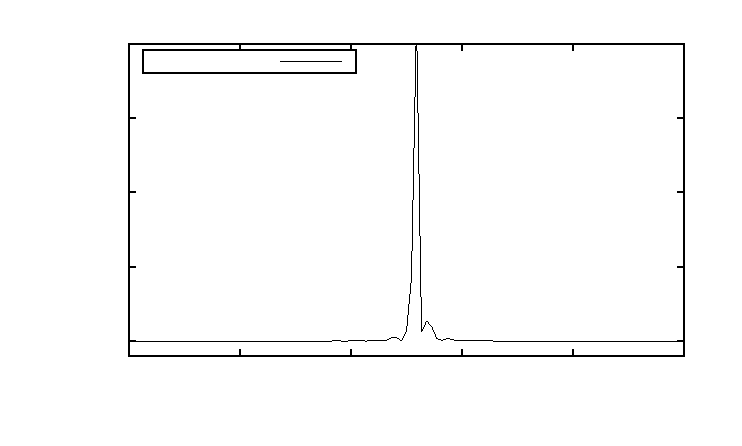
\includegraphics{led-laser-spec}}%
    \gplfronttext
  \end{picture}%
\endgroup

				\caption{Spektrum einer roten Laser-LED aufgenommen mit $100000$ Samples und $1000 \unit{sps}$}
				\label{fig:rot-laser-led}
			\end{figure}

			\begin{figure}[htb]
				\centering
				% GNUPLOT: LaTeX picture with Postscript
\begingroup
  \makeatletter
  \providecommand\color[2][]{%
    \GenericError{(gnuplot) \space\space\space\@spaces}{%
      Package color not loaded in conjunction with
      terminal option `colourtext'%
    }{See the gnuplot documentation for explanation.%
    }{Either use 'blacktext' in gnuplot or load the package
      color.sty in LaTeX.}%
    \renewcommand\color[2][]{}%
  }%
  \providecommand\includegraphics[2][]{%
    \GenericError{(gnuplot) \space\space\space\@spaces}{%
      Package graphicx or graphics not loaded%
    }{See the gnuplot documentation for explanation.%
    }{The gnuplot epslatex terminal needs graphicx.sty or graphics.sty.}%
    \renewcommand\includegraphics[2][]{}%
  }%
  \providecommand\rotatebox[2]{#2}%
  \@ifundefined{ifGPcolor}{%
    \newif\ifGPcolor
    \GPcolorfalse
  }{}%
  \@ifundefined{ifGPblacktext}{%
    \newif\ifGPblacktext
    \GPblacktexttrue
  }{}%
  % define a \g@addto@macro without @ in the name:
  \let\gplgaddtomacro\g@addto@macro
  % define empty templates for all commands taking text:
  \gdef\gplbacktext{}%
  \gdef\gplfronttext{}%
  \makeatother
  \ifGPblacktext
    % no textcolor at all
    \def\colorrgb#1{}%
    \def\colorgray#1{}%
  \else
    % gray or color?
    \ifGPcolor
      \def\colorrgb#1{\color[rgb]{#1}}%
      \def\colorgray#1{\color[gray]{#1}}%
      \expandafter\def\csname LTw\endcsname{\color{white}}%
      \expandafter\def\csname LTb\endcsname{\color{black}}%
      \expandafter\def\csname LTa\endcsname{\color{black}}%
      \expandafter\def\csname LT0\endcsname{\color[rgb]{1,0,0}}%
      \expandafter\def\csname LT1\endcsname{\color[rgb]{0,1,0}}%
      \expandafter\def\csname LT2\endcsname{\color[rgb]{0,0,1}}%
      \expandafter\def\csname LT3\endcsname{\color[rgb]{1,0,1}}%
      \expandafter\def\csname LT4\endcsname{\color[rgb]{0,1,1}}%
      \expandafter\def\csname LT5\endcsname{\color[rgb]{1,1,0}}%
      \expandafter\def\csname LT6\endcsname{\color[rgb]{0,0,0}}%
      \expandafter\def\csname LT7\endcsname{\color[rgb]{1,0.3,0}}%
      \expandafter\def\csname LT8\endcsname{\color[rgb]{0.5,0.5,0.5}}%
    \else
      % gray
      \def\colorrgb#1{\color{black}}%
      \def\colorgray#1{\color[gray]{#1}}%
      \expandafter\def\csname LTw\endcsname{\color{white}}%
      \expandafter\def\csname LTb\endcsname{\color{black}}%
      \expandafter\def\csname LTa\endcsname{\color{black}}%
      \expandafter\def\csname LT0\endcsname{\color{black}}%
      \expandafter\def\csname LT1\endcsname{\color{black}}%
      \expandafter\def\csname LT2\endcsname{\color{black}}%
      \expandafter\def\csname LT3\endcsname{\color{black}}%
      \expandafter\def\csname LT4\endcsname{\color{black}}%
      \expandafter\def\csname LT5\endcsname{\color{black}}%
      \expandafter\def\csname LT6\endcsname{\color{black}}%
      \expandafter\def\csname LT7\endcsname{\color{black}}%
      \expandafter\def\csname LT8\endcsname{\color{black}}%
    \fi
  \fi
  \setlength{\unitlength}{0.0500bp}%
  \begin{picture}(6802.00,3968.00)%
    \gplgaddtomacro\gplbacktext{%
      \csname LTb\endcsname%
      \put(946,801){\makebox(0,0)[r]{\strut{} 0}}%
      \put(946,1284){\makebox(0,0)[r]{\strut{} 0.5}}%
      \put(946,1768){\makebox(0,0)[r]{\strut{} 1}}%
      \put(946,2252){\makebox(0,0)[r]{\strut{} 1.5}}%
      \put(946,2736){\makebox(0,0)[r]{\strut{} 2}}%
      \put(946,3219){\makebox(0,0)[r]{\strut{} 2.5}}%
      \put(946,3703){\makebox(0,0)[r]{\strut{} 3}}%
      \put(1078,484){\makebox(0,0){\strut{} 520}}%
      \put(2410,484){\makebox(0,0){\strut{} 525}}%
      \put(3742,484){\makebox(0,0){\strut{} 530}}%
      \put(5073,484){\makebox(0,0){\strut{} 535}}%
      \put(6405,484){\makebox(0,0){\strut{} 540}}%
      \put(176,2203){\rotatebox{-270}{\makebox(0,0){\strut{}Intensität}}}%
      \put(3741,154){\makebox(0,0){\strut{}Wellenlänge $\lambda \ [\unit{nm}]$}}%
    }%
    \gplgaddtomacro\gplfronttext{%
      \csname LTb\endcsname%
      \put(2398,3530){\makebox(0,0)[r]{\strut{}Messwerte}}%
    }%
    \gplbacktext
    \put(0,0){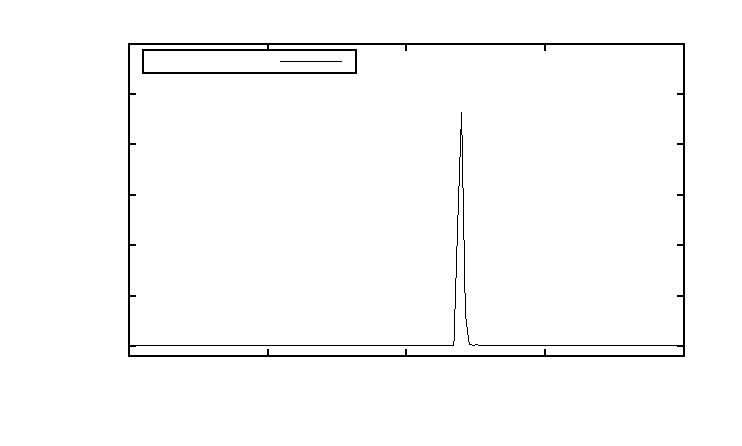
\includegraphics{g-laser-spec}}%
    \gplfronttext
  \end{picture}%
\endgroup

				\caption{Spektrum eines grünen, frequenzverdoppelten Nd:YAG Lasers aufgenommen mit $100000$ Samples und $500 \unit{sps}$}
				\label{fig:nd-yaq-laser}
			\end{figure}

		% subsubsection spektrum_led_und_gaslaser (end)

		\subsubsection{Spektrum Natrium- und Quecksilberdampflampe} % (fold)
		\label{ssub:spektrum_natrium_und_quecksilberdampflampe}

			Um die Eignung des FS zur Untersuchung von Atomspektren zu überprüfen wurden die Intensitätsverteilungen von Natriumlampe und Quecksilberdampflampe aufgenommen und vermessen.
			Graph \ref{fig:na-spec} zeigt den charakteristischen Doppelpeak von Na bei ca. $589.0$ und $589.5 \unit{nm}$.
			Das der recht schmale Doppelpeak noch getrennt zu sehen ist, liegt wiederum am Auflösevermögen.
			Es beträgt im gezeigten Bild etwa:
			\[ \frac{200 \unit{s} \cdot 10 \,\mu\m{m}s^{-1}}{589 \unit{nm}} \approx 3400 \qquad > \qquad \frac{\lambda}{\Delta \lambda} = 1178 \]

			Das Quecksilberspektrum zeigt über einen sehr großen Bereich detailliert alle Peaks.
			Die ermittelten Wellenlängen stimmen auf den Nanometer mit dem Vergleichsspektrum aus Abschnitt \ref{sec:hg_spektrum} überein.
			\begin{table}[h]
				\begin{tabular}{r|rrrrr}
					Messwerte $[\unit{nm}]$ & $579.1$ & $576.9$ & $546.0$ & $435.8$ & $404.6$ \\
					\hline
					Tabellenwerte $[\unit{nm}]$ & $579$ & $577$ & $546.1$ & $435.8$ & $405$
				\end{tabular}
				\caption{Spektrallinien des Quecksilbers}
			\end{table}
			Allerdings erkennt man das im Bereich zwischen $436$ und $546 \unit{nm}$ etliche Spektrallinien fehlen, was mit ihrer zu geringen Intensität zu erklären ist.
			Auch hier genügt die Auflösung wieder für die zwei eng benachbarten Linien bei $577$ und $579 \unit{nm}$.


			\begin{figure}[htb]
				\centering
				% GNUPLOT: LaTeX picture with Postscript
\begingroup
  \makeatletter
  \providecommand\color[2][]{%
    \GenericError{(gnuplot) \space\space\space\@spaces}{%
      Package color not loaded in conjunction with
      terminal option `colourtext'%
    }{See the gnuplot documentation for explanation.%
    }{Either use 'blacktext' in gnuplot or load the package
      color.sty in LaTeX.}%
    \renewcommand\color[2][]{}%
  }%
  \providecommand\includegraphics[2][]{%
    \GenericError{(gnuplot) \space\space\space\@spaces}{%
      Package graphicx or graphics not loaded%
    }{See the gnuplot documentation for explanation.%
    }{The gnuplot epslatex terminal needs graphicx.sty or graphics.sty.}%
    \renewcommand\includegraphics[2][]{}%
  }%
  \providecommand\rotatebox[2]{#2}%
  \@ifundefined{ifGPcolor}{%
    \newif\ifGPcolor
    \GPcolorfalse
  }{}%
  \@ifundefined{ifGPblacktext}{%
    \newif\ifGPblacktext
    \GPblacktexttrue
  }{}%
  % define a \g@addto@macro without @ in the name:
  \let\gplgaddtomacro\g@addto@macro
  % define empty templates for all commands taking text:
  \gdef\gplbacktext{}%
  \gdef\gplfronttext{}%
  \makeatother
  \ifGPblacktext
    % no textcolor at all
    \def\colorrgb#1{}%
    \def\colorgray#1{}%
  \else
    % gray or color?
    \ifGPcolor
      \def\colorrgb#1{\color[rgb]{#1}}%
      \def\colorgray#1{\color[gray]{#1}}%
      \expandafter\def\csname LTw\endcsname{\color{white}}%
      \expandafter\def\csname LTb\endcsname{\color{black}}%
      \expandafter\def\csname LTa\endcsname{\color{black}}%
      \expandafter\def\csname LT0\endcsname{\color[rgb]{1,0,0}}%
      \expandafter\def\csname LT1\endcsname{\color[rgb]{0,1,0}}%
      \expandafter\def\csname LT2\endcsname{\color[rgb]{0,0,1}}%
      \expandafter\def\csname LT3\endcsname{\color[rgb]{1,0,1}}%
      \expandafter\def\csname LT4\endcsname{\color[rgb]{0,1,1}}%
      \expandafter\def\csname LT5\endcsname{\color[rgb]{1,1,0}}%
      \expandafter\def\csname LT6\endcsname{\color[rgb]{0,0,0}}%
      \expandafter\def\csname LT7\endcsname{\color[rgb]{1,0.3,0}}%
      \expandafter\def\csname LT8\endcsname{\color[rgb]{0.5,0.5,0.5}}%
    \else
      % gray
      \def\colorrgb#1{\color{black}}%
      \def\colorgray#1{\color[gray]{#1}}%
      \expandafter\def\csname LTw\endcsname{\color{white}}%
      \expandafter\def\csname LTb\endcsname{\color{black}}%
      \expandafter\def\csname LTa\endcsname{\color{black}}%
      \expandafter\def\csname LT0\endcsname{\color{black}}%
      \expandafter\def\csname LT1\endcsname{\color{black}}%
      \expandafter\def\csname LT2\endcsname{\color{black}}%
      \expandafter\def\csname LT3\endcsname{\color{black}}%
      \expandafter\def\csname LT4\endcsname{\color{black}}%
      \expandafter\def\csname LT5\endcsname{\color{black}}%
      \expandafter\def\csname LT6\endcsname{\color{black}}%
      \expandafter\def\csname LT7\endcsname{\color{black}}%
      \expandafter\def\csname LT8\endcsname{\color{black}}%
    \fi
  \fi
  \setlength{\unitlength}{0.0500bp}%
  \begin{picture}(6802.00,3968.00)%
    \gplgaddtomacro\gplbacktext{%
      \csname LTb\endcsname%
      \put(814,724){\makebox(0,0)[r]{\strut{} 0}}%
      \put(814,1121){\makebox(0,0)[r]{\strut{} 2}}%
      \put(814,1518){\makebox(0,0)[r]{\strut{} 4}}%
      \put(814,1916){\makebox(0,0)[r]{\strut{} 6}}%
      \put(814,2313){\makebox(0,0)[r]{\strut{} 8}}%
      \put(814,2710){\makebox(0,0)[r]{\strut{} 10}}%
      \put(814,3107){\makebox(0,0)[r]{\strut{} 12}}%
      \put(814,3504){\makebox(0,0)[r]{\strut{} 14}}%
      \put(946,484){\makebox(0,0){\strut{} 585}}%
      \put(1726,484){\makebox(0,0){\strut{} 586}}%
      \put(2506,484){\makebox(0,0){\strut{} 587}}%
      \put(3286,484){\makebox(0,0){\strut{} 588}}%
      \put(4065,484){\makebox(0,0){\strut{} 589}}%
      \put(4845,484){\makebox(0,0){\strut{} 590}}%
      \put(5625,484){\makebox(0,0){\strut{} 591}}%
      \put(6405,484){\makebox(0,0){\strut{} 592}}%
      \put(176,2203){\rotatebox{-270}{\makebox(0,0){\strut{}Intensität}}}%
      \put(3675,154){\makebox(0,0){\strut{}Wellenlänge $\lambda \ [\unit{nm}]$}}%
    }%
    \gplgaddtomacro\gplfronttext{%
      \csname LTb\endcsname%
      \put(2266,3530){\makebox(0,0)[r]{\strut{}Messwerte}}%
    }%
    \gplbacktext
    \put(0,0){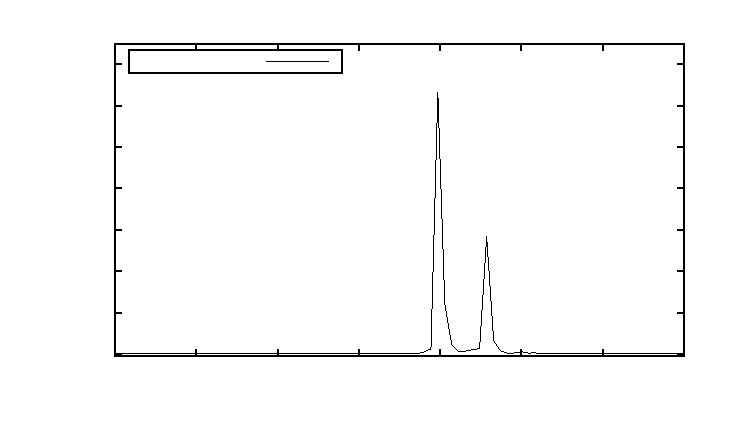
\includegraphics{na-dd}}%
    \gplfronttext
  \end{picture}%
\endgroup

				\caption{Vergrößerter Ausschnitt aus dem Spektrum der Na-Lampe mit typischer Doppel-D-Linie,
				Aufnahme mit $200000$ Samples und $1000 \unit{sps}$}
				\label{fig:na-spec}
			\end{figure}

			\begin{figure}[htb]
				\centering
				% GNUPLOT: LaTeX picture with Postscript
\begingroup
  \makeatletter
  \providecommand\color[2][]{%
    \GenericError{(gnuplot) \space\space\space\@spaces}{%
      Package color not loaded in conjunction with
      terminal option `colourtext'%
    }{See the gnuplot documentation for explanation.%
    }{Either use 'blacktext' in gnuplot or load the package
      color.sty in LaTeX.}%
    \renewcommand\color[2][]{}%
  }%
  \providecommand\includegraphics[2][]{%
    \GenericError{(gnuplot) \space\space\space\@spaces}{%
      Package graphicx or graphics not loaded%
    }{See the gnuplot documentation for explanation.%
    }{The gnuplot epslatex terminal needs graphicx.sty or graphics.sty.}%
    \renewcommand\includegraphics[2][]{}%
  }%
  \providecommand\rotatebox[2]{#2}%
  \@ifundefined{ifGPcolor}{%
    \newif\ifGPcolor
    \GPcolorfalse
  }{}%
  \@ifundefined{ifGPblacktext}{%
    \newif\ifGPblacktext
    \GPblacktexttrue
  }{}%
  % define a \g@addto@macro without @ in the name:
  \let\gplgaddtomacro\g@addto@macro
  % define empty templates for all commands taking text:
  \gdef\gplbacktext{}%
  \gdef\gplfronttext{}%
  \makeatother
  \ifGPblacktext
    % no textcolor at all
    \def\colorrgb#1{}%
    \def\colorgray#1{}%
  \else
    % gray or color?
    \ifGPcolor
      \def\colorrgb#1{\color[rgb]{#1}}%
      \def\colorgray#1{\color[gray]{#1}}%
      \expandafter\def\csname LTw\endcsname{\color{white}}%
      \expandafter\def\csname LTb\endcsname{\color{black}}%
      \expandafter\def\csname LTa\endcsname{\color{black}}%
      \expandafter\def\csname LT0\endcsname{\color[rgb]{1,0,0}}%
      \expandafter\def\csname LT1\endcsname{\color[rgb]{0,1,0}}%
      \expandafter\def\csname LT2\endcsname{\color[rgb]{0,0,1}}%
      \expandafter\def\csname LT3\endcsname{\color[rgb]{1,0,1}}%
      \expandafter\def\csname LT4\endcsname{\color[rgb]{0,1,1}}%
      \expandafter\def\csname LT5\endcsname{\color[rgb]{1,1,0}}%
      \expandafter\def\csname LT6\endcsname{\color[rgb]{0,0,0}}%
      \expandafter\def\csname LT7\endcsname{\color[rgb]{1,0.3,0}}%
      \expandafter\def\csname LT8\endcsname{\color[rgb]{0.5,0.5,0.5}}%
    \else
      % gray
      \def\colorrgb#1{\color{black}}%
      \def\colorgray#1{\color[gray]{#1}}%
      \expandafter\def\csname LTw\endcsname{\color{white}}%
      \expandafter\def\csname LTb\endcsname{\color{black}}%
      \expandafter\def\csname LTa\endcsname{\color{black}}%
      \expandafter\def\csname LT0\endcsname{\color{black}}%
      \expandafter\def\csname LT1\endcsname{\color{black}}%
      \expandafter\def\csname LT2\endcsname{\color{black}}%
      \expandafter\def\csname LT3\endcsname{\color{black}}%
      \expandafter\def\csname LT4\endcsname{\color{black}}%
      \expandafter\def\csname LT5\endcsname{\color{black}}%
      \expandafter\def\csname LT6\endcsname{\color{black}}%
      \expandafter\def\csname LT7\endcsname{\color{black}}%
      \expandafter\def\csname LT8\endcsname{\color{black}}%
    \fi
  \fi
  \setlength{\unitlength}{0.0500bp}%
  \begin{picture}(6802.00,3968.00)%
    \gplgaddtomacro\gplbacktext{%
      \csname LTb\endcsname%
      \put(682,763){\makebox(0,0)[r]{\strut{} 0}}%
      \put(682,1351){\makebox(0,0)[r]{\strut{} 1}}%
      \put(682,1939){\makebox(0,0)[r]{\strut{} 2}}%
      \put(682,2527){\makebox(0,0)[r]{\strut{} 3}}%
      \put(682,3115){\makebox(0,0)[r]{\strut{} 4}}%
      \put(682,3703){\makebox(0,0)[r]{\strut{} 5}}%
      \put(1322,484){\makebox(0,0){\strut{} 400}}%
      \put(2593,484){\makebox(0,0){\strut{} 450}}%
      \put(3864,484){\makebox(0,0){\strut{} 500}}%
      \put(5134,484){\makebox(0,0){\strut{} 550}}%
      \put(6405,484){\makebox(0,0){\strut{} 600}}%
      \put(176,2203){\rotatebox{-270}{\makebox(0,0){\strut{}Intensität}}}%
      \put(3609,154){\makebox(0,0){\strut{}Wellenlänge $\lambda \ [\unit{nm}]$}}%
    }%
    \gplgaddtomacro\gplfronttext{%
      \csname LTb\endcsname%
      \put(3776,3530){\makebox(0,0)[r]{\strut{}Messwerte}}%
    }%
    \gplbacktext
    \put(0,0){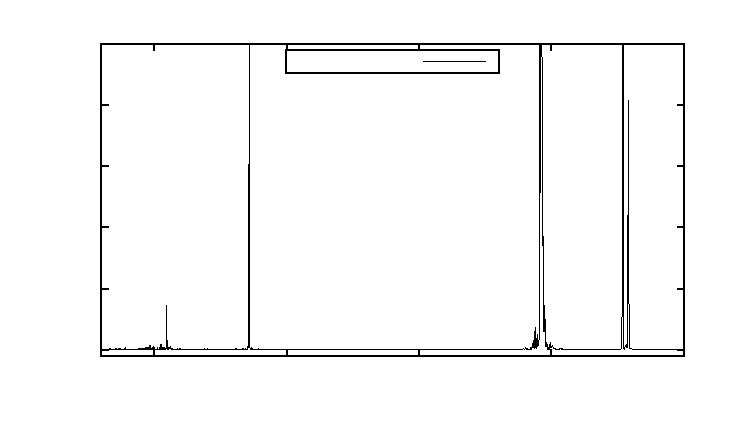
\includegraphics{hg-spec}}%
    \gplfronttext
  \end{picture}%
\endgroup

				\caption{Breiter Bereich des Spektrums einer Hg-Dampflampe, 
				Aufnahme mit $100000$ Samples und $1000 \unit{sps}$}
				\label{fig:hg.spec}
			\end{figure}
			
		% subsubsection spektrum_natrium_und_quecksilberdampflampe (end)


		\subsubsection{Glühlampenspektrum und Detektorbandlücke} % (fold)
		\label{ssub:gl_hlampenspektrum}

			Speziell zur Analyse für Infrarotspektren wird häufig ein FS verwendet, da hier die Motoreinstellung leichter auf Wellenlängengenauigkeit einzustellen ist.
			Das Spektrum der Wolfram-Glühlampe ist in Abbildung \ref{fig:lamp-si} zu sehen.
			Hier wurde zur Aufnahme ein Si-Detektor mit einer Bandlücke von $1.12 \unit{eV}$ verwendet.\footnote{Quelle: Hunklinger Festkörperphysik S. 413}
			Offenbar reicht hier das Spektrum bis etwa $1070 \unit{nm}$ und hat sein Maximum im roten bei $900$.
			Die selbe Quelle mit einem PbSe-Detektor ausgewertet, wie in Abbildung \ref{fig:lamp-pbse} gezeigt, liefert ein ganz anderes Spektrum.
			Hier scheint das Spektrum bei $1000 \unit{nm}$ gerade erst anzufangen und hat sein Maximum bei $1650$ um dann weit im Infraroten bei ca. $2600 \unit{nm}$ abzuflachen.
			Die Ursache für den frühen Abbruch im Si-aufgenommenen Spektrum liegt an der relativ großen Bandlücke des Silizium Halbleiters.
			Mit Hilfe der Bandlückenenergie $E_\m{gap}$ kann die größtmögliche noch zu messende Wellenlänge bestimmt werden:
			\[ \lambda _ \m{max} = \frac{h c}{E_\m{gap}} \approx 1100 \unit{nm}\]
			Im Falle von PbSe mit $E_\m{gap} = 0.278 \unit{eV}$ ergibt sich analog\footnote{Quelle: \url{http://link.springer.com/chapter/10.1007/10681727_890#page-1}}
			\[ \lambda _ \m{max} \approx 4460 \unit{nm}\]
			Wie wir sehen liegt im Fall des Si-Detektors die Bandlückenenergie größer als die Energie der langwelligen Photonen, weshalb das Spektrum hier abbricht.
			Im Fall der PbSe-Detektors liegt $\lambda _ \m{max}$ weit außerhalb der Emission.
			Das Spektrum der Halogen-Lampe aus Abbildung \ref{fig:halo-pbse} zeigt einen ganz ähnlichen Verlauf mit Maximum in etwa an der gleichen Stelle.
			Die Halogen-Lampe wurde im weiteren Verlauf statt der Glühlampe verwendet weil sie sich besser eignete und sie nicht ansteuerbar war, weshalb sie stets die gleiche Leistung und das gleiche Spektrum hatte (und vor allem weil die Glühlampe durchgebrannt war).
			Beide Spektren (vom PbSe-Detektor) zeigen den typischen Verlauf eines schwarzen Strahlers.
			Es ist bemerkenswert, dass beide Lampen ihr eigentliches Maximum weit außerhalb des sichtbaren Lichtes haben, was die Vermutung über den schlechten Wirkungsgrad bestätigt.
			Der Knick bei ca. $1410 \unit{nm}$ entsteht durch das Absorptionsverhalten von Wasser und Kohlenstoffdioxid in der Atmosphäre, näheres dazu unter Abschnitt \ref{ssub:absorbtionsspektren_von_wasser_und_benzol}.


			\begin{figure}[htb]
				\centering
				% GNUPLOT: LaTeX picture with Postscript
\begingroup
  \makeatletter
  \providecommand\color[2][]{%
    \GenericError{(gnuplot) \space\space\space\@spaces}{%
      Package color not loaded in conjunction with
      terminal option `colourtext'%
    }{See the gnuplot documentation for explanation.%
    }{Either use 'blacktext' in gnuplot or load the package
      color.sty in LaTeX.}%
    \renewcommand\color[2][]{}%
  }%
  \providecommand\includegraphics[2][]{%
    \GenericError{(gnuplot) \space\space\space\@spaces}{%
      Package graphicx or graphics not loaded%
    }{See the gnuplot documentation for explanation.%
    }{The gnuplot epslatex terminal needs graphicx.sty or graphics.sty.}%
    \renewcommand\includegraphics[2][]{}%
  }%
  \providecommand\rotatebox[2]{#2}%
  \@ifundefined{ifGPcolor}{%
    \newif\ifGPcolor
    \GPcolorfalse
  }{}%
  \@ifundefined{ifGPblacktext}{%
    \newif\ifGPblacktext
    \GPblacktexttrue
  }{}%
  % define a \g@addto@macro without @ in the name:
  \let\gplgaddtomacro\g@addto@macro
  % define empty templates for all commands taking text:
  \gdef\gplbacktext{}%
  \gdef\gplfronttext{}%
  \makeatother
  \ifGPblacktext
    % no textcolor at all
    \def\colorrgb#1{}%
    \def\colorgray#1{}%
  \else
    % gray or color?
    \ifGPcolor
      \def\colorrgb#1{\color[rgb]{#1}}%
      \def\colorgray#1{\color[gray]{#1}}%
      \expandafter\def\csname LTw\endcsname{\color{white}}%
      \expandafter\def\csname LTb\endcsname{\color{black}}%
      \expandafter\def\csname LTa\endcsname{\color{black}}%
      \expandafter\def\csname LT0\endcsname{\color[rgb]{1,0,0}}%
      \expandafter\def\csname LT1\endcsname{\color[rgb]{0,1,0}}%
      \expandafter\def\csname LT2\endcsname{\color[rgb]{0,0,1}}%
      \expandafter\def\csname LT3\endcsname{\color[rgb]{1,0,1}}%
      \expandafter\def\csname LT4\endcsname{\color[rgb]{0,1,1}}%
      \expandafter\def\csname LT5\endcsname{\color[rgb]{1,1,0}}%
      \expandafter\def\csname LT6\endcsname{\color[rgb]{0,0,0}}%
      \expandafter\def\csname LT7\endcsname{\color[rgb]{1,0.3,0}}%
      \expandafter\def\csname LT8\endcsname{\color[rgb]{0.5,0.5,0.5}}%
    \else
      % gray
      \def\colorrgb#1{\color{black}}%
      \def\colorgray#1{\color[gray]{#1}}%
      \expandafter\def\csname LTw\endcsname{\color{white}}%
      \expandafter\def\csname LTb\endcsname{\color{black}}%
      \expandafter\def\csname LTa\endcsname{\color{black}}%
      \expandafter\def\csname LT0\endcsname{\color{black}}%
      \expandafter\def\csname LT1\endcsname{\color{black}}%
      \expandafter\def\csname LT2\endcsname{\color{black}}%
      \expandafter\def\csname LT3\endcsname{\color{black}}%
      \expandafter\def\csname LT4\endcsname{\color{black}}%
      \expandafter\def\csname LT5\endcsname{\color{black}}%
      \expandafter\def\csname LT6\endcsname{\color{black}}%
      \expandafter\def\csname LT7\endcsname{\color{black}}%
      \expandafter\def\csname LT8\endcsname{\color{black}}%
    \fi
  \fi
  \setlength{\unitlength}{0.0500bp}%
  \begin{picture}(6802.00,3968.00)%
    \gplgaddtomacro\gplbacktext{%
      \csname LTb\endcsname%
      \put(946,954){\makebox(0,0)[r]{\strut{} 0}}%
      \put(946,1454){\makebox(0,0)[r]{\strut{} 0.2}}%
      \put(946,1954){\makebox(0,0)[r]{\strut{} 0.4}}%
      \put(946,2453){\makebox(0,0)[r]{\strut{} 0.6}}%
      \put(946,2953){\makebox(0,0)[r]{\strut{} 0.8}}%
      \put(946,3453){\makebox(0,0)[r]{\strut{} 1}}%
      \put(1078,484){\makebox(0,0){\strut{} 400}}%
      \put(1744,484){\makebox(0,0){\strut{} 500}}%
      \put(2410,484){\makebox(0,0){\strut{} 600}}%
      \put(3076,484){\makebox(0,0){\strut{} 700}}%
      \put(3742,484){\makebox(0,0){\strut{} 800}}%
      \put(4407,484){\makebox(0,0){\strut{} 900}}%
      \put(5073,484){\makebox(0,0){\strut{} 1000}}%
      \put(5739,484){\makebox(0,0){\strut{} 1100}}%
      \put(6405,484){\makebox(0,0){\strut{} 1200}}%
      \put(176,2203){\rotatebox{-270}{\makebox(0,0){\strut{}Intensität}}}%
      \put(3741,154){\makebox(0,0){\strut{}Wellenlänge $\lambda \ [\unit{nm}]$}}%
    }%
    \gplgaddtomacro\gplfronttext{%
      \csname LTb\endcsname%
      \put(2398,3530){\makebox(0,0)[r]{\strut{}Messwerte}}%
    }%
    \gplbacktext
    \put(0,0){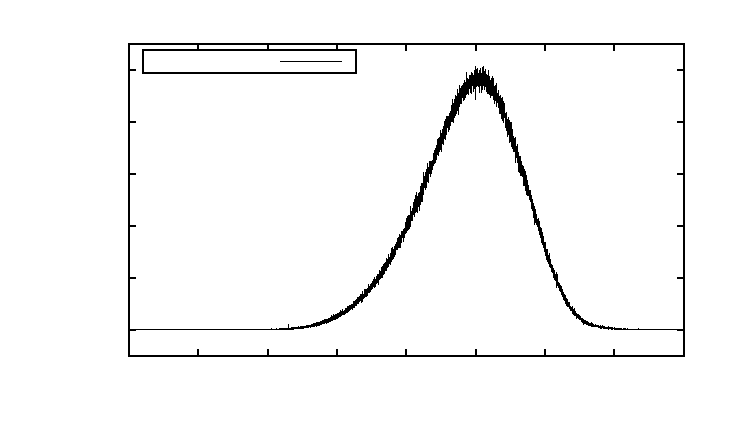
\includegraphics{lamp-spec}}%
    \gplfronttext
  \end{picture}%
\endgroup

				\caption{Spektrum einer herkömmlichen Wolfram-Glühbirne aufgezeichnet mit einem Siliziumdetektor 
				sowie $100000$ Samples und $500 \unit{sps}$}
				\label{fig:lamp-si}
			\end{figure}

			\begin{figure}[htb]
				\centering
				% GNUPLOT: LaTeX picture with Postscript
\begingroup
  \makeatletter
  \providecommand\color[2][]{%
    \GenericError{(gnuplot) \space\space\space\@spaces}{%
      Package color not loaded in conjunction with
      terminal option `colourtext'%
    }{See the gnuplot documentation for explanation.%
    }{Either use 'blacktext' in gnuplot or load the package
      color.sty in LaTeX.}%
    \renewcommand\color[2][]{}%
  }%
  \providecommand\includegraphics[2][]{%
    \GenericError{(gnuplot) \space\space\space\@spaces}{%
      Package graphicx or graphics not loaded%
    }{See the gnuplot documentation for explanation.%
    }{The gnuplot epslatex terminal needs graphicx.sty or graphics.sty.}%
    \renewcommand\includegraphics[2][]{}%
  }%
  \providecommand\rotatebox[2]{#2}%
  \@ifundefined{ifGPcolor}{%
    \newif\ifGPcolor
    \GPcolorfalse
  }{}%
  \@ifundefined{ifGPblacktext}{%
    \newif\ifGPblacktext
    \GPblacktexttrue
  }{}%
  % define a \g@addto@macro without @ in the name:
  \let\gplgaddtomacro\g@addto@macro
  % define empty templates for all commands taking text:
  \gdef\gplbacktext{}%
  \gdef\gplfronttext{}%
  \makeatother
  \ifGPblacktext
    % no textcolor at all
    \def\colorrgb#1{}%
    \def\colorgray#1{}%
  \else
    % gray or color?
    \ifGPcolor
      \def\colorrgb#1{\color[rgb]{#1}}%
      \def\colorgray#1{\color[gray]{#1}}%
      \expandafter\def\csname LTw\endcsname{\color{white}}%
      \expandafter\def\csname LTb\endcsname{\color{black}}%
      \expandafter\def\csname LTa\endcsname{\color{black}}%
      \expandafter\def\csname LT0\endcsname{\color[rgb]{1,0,0}}%
      \expandafter\def\csname LT1\endcsname{\color[rgb]{0,1,0}}%
      \expandafter\def\csname LT2\endcsname{\color[rgb]{0,0,1}}%
      \expandafter\def\csname LT3\endcsname{\color[rgb]{1,0,1}}%
      \expandafter\def\csname LT4\endcsname{\color[rgb]{0,1,1}}%
      \expandafter\def\csname LT5\endcsname{\color[rgb]{1,1,0}}%
      \expandafter\def\csname LT6\endcsname{\color[rgb]{0,0,0}}%
      \expandafter\def\csname LT7\endcsname{\color[rgb]{1,0.3,0}}%
      \expandafter\def\csname LT8\endcsname{\color[rgb]{0.5,0.5,0.5}}%
    \else
      % gray
      \def\colorrgb#1{\color{black}}%
      \def\colorgray#1{\color[gray]{#1}}%
      \expandafter\def\csname LTw\endcsname{\color{white}}%
      \expandafter\def\csname LTb\endcsname{\color{black}}%
      \expandafter\def\csname LTa\endcsname{\color{black}}%
      \expandafter\def\csname LT0\endcsname{\color{black}}%
      \expandafter\def\csname LT1\endcsname{\color{black}}%
      \expandafter\def\csname LT2\endcsname{\color{black}}%
      \expandafter\def\csname LT3\endcsname{\color{black}}%
      \expandafter\def\csname LT4\endcsname{\color{black}}%
      \expandafter\def\csname LT5\endcsname{\color{black}}%
      \expandafter\def\csname LT6\endcsname{\color{black}}%
      \expandafter\def\csname LT7\endcsname{\color{black}}%
      \expandafter\def\csname LT8\endcsname{\color{black}}%
    \fi
  \fi
  \setlength{\unitlength}{0.0500bp}%
  \begin{picture}(6802.00,3968.00)%
    \gplgaddtomacro\gplbacktext{%
      \csname LTb\endcsname%
      \put(946,954){\makebox(0,0)[r]{\strut{} 0}}%
      \put(946,1454){\makebox(0,0)[r]{\strut{} 0.2}}%
      \put(946,1954){\makebox(0,0)[r]{\strut{} 0.4}}%
      \put(946,2453){\makebox(0,0)[r]{\strut{} 0.6}}%
      \put(946,2953){\makebox(0,0)[r]{\strut{} 0.8}}%
      \put(946,3453){\makebox(0,0)[r]{\strut{} 1}}%
      \put(1283,484){\makebox(0,0){\strut{} 500}}%
      \put(2307,484){\makebox(0,0){\strut{} 1000}}%
      \put(3332,484){\makebox(0,0){\strut{} 1500}}%
      \put(4356,484){\makebox(0,0){\strut{} 2000}}%
      \put(5381,484){\makebox(0,0){\strut{} 2500}}%
      \put(6405,484){\makebox(0,0){\strut{} 3000}}%
      \put(176,2203){\rotatebox{-270}{\makebox(0,0){\strut{}Intensität}}}%
      \put(3741,154){\makebox(0,0){\strut{}Wellenlänge $\lambda \ [\unit{nm}]$}}%
    }%
    \gplgaddtomacro\gplfronttext{%
      \csname LTb\endcsname%
      \put(2398,3530){\makebox(0,0)[r]{\strut{}Messwerte}}%
    }%
    \gplbacktext
    \put(0,0){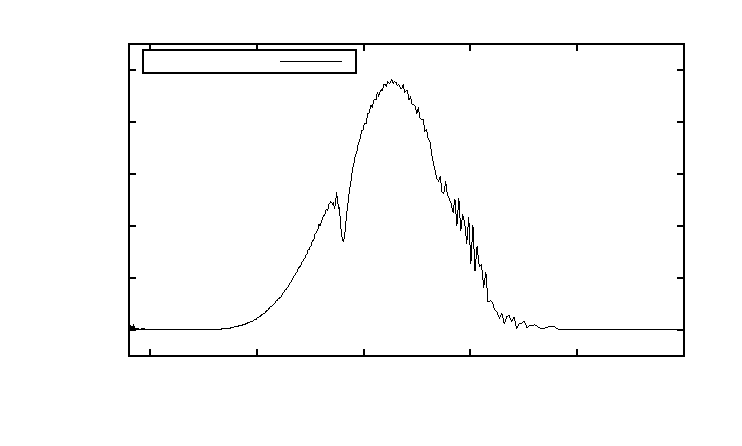
\includegraphics{lamp-pbse-spec}}%
    \gplfronttext
  \end{picture}%
\endgroup

				\caption{Spektrum einer herkömmlichen Wolfram-Glühbirne aufgezeichnet mit einem Bleiseleniddetektor 
				sowie $100000$ Samples und $500 \unit{sps}$}
				\label{fig:lamp-pbse}
			\end{figure}

			\begin{figure}[htb]
				\centering
				% GNUPLOT: LaTeX picture with Postscript
\begingroup
  \makeatletter
  \providecommand\color[2][]{%
    \GenericError{(gnuplot) \space\space\space\@spaces}{%
      Package color not loaded in conjunction with
      terminal option `colourtext'%
    }{See the gnuplot documentation for explanation.%
    }{Either use 'blacktext' in gnuplot or load the package
      color.sty in LaTeX.}%
    \renewcommand\color[2][]{}%
  }%
  \providecommand\includegraphics[2][]{%
    \GenericError{(gnuplot) \space\space\space\@spaces}{%
      Package graphicx or graphics not loaded%
    }{See the gnuplot documentation for explanation.%
    }{The gnuplot epslatex terminal needs graphicx.sty or graphics.sty.}%
    \renewcommand\includegraphics[2][]{}%
  }%
  \providecommand\rotatebox[2]{#2}%
  \@ifundefined{ifGPcolor}{%
    \newif\ifGPcolor
    \GPcolorfalse
  }{}%
  \@ifundefined{ifGPblacktext}{%
    \newif\ifGPblacktext
    \GPblacktexttrue
  }{}%
  % define a \g@addto@macro without @ in the name:
  \let\gplgaddtomacro\g@addto@macro
  % define empty templates for all commands taking text:
  \gdef\gplbacktext{}%
  \gdef\gplfronttext{}%
  \makeatother
  \ifGPblacktext
    % no textcolor at all
    \def\colorrgb#1{}%
    \def\colorgray#1{}%
  \else
    % gray or color?
    \ifGPcolor
      \def\colorrgb#1{\color[rgb]{#1}}%
      \def\colorgray#1{\color[gray]{#1}}%
      \expandafter\def\csname LTw\endcsname{\color{white}}%
      \expandafter\def\csname LTb\endcsname{\color{black}}%
      \expandafter\def\csname LTa\endcsname{\color{black}}%
      \expandafter\def\csname LT0\endcsname{\color[rgb]{1,0,0}}%
      \expandafter\def\csname LT1\endcsname{\color[rgb]{0,1,0}}%
      \expandafter\def\csname LT2\endcsname{\color[rgb]{0,0,1}}%
      \expandafter\def\csname LT3\endcsname{\color[rgb]{1,0,1}}%
      \expandafter\def\csname LT4\endcsname{\color[rgb]{0,1,1}}%
      \expandafter\def\csname LT5\endcsname{\color[rgb]{1,1,0}}%
      \expandafter\def\csname LT6\endcsname{\color[rgb]{0,0,0}}%
      \expandafter\def\csname LT7\endcsname{\color[rgb]{1,0.3,0}}%
      \expandafter\def\csname LT8\endcsname{\color[rgb]{0.5,0.5,0.5}}%
    \else
      % gray
      \def\colorrgb#1{\color{black}}%
      \def\colorgray#1{\color[gray]{#1}}%
      \expandafter\def\csname LTw\endcsname{\color{white}}%
      \expandafter\def\csname LTb\endcsname{\color{black}}%
      \expandafter\def\csname LTa\endcsname{\color{black}}%
      \expandafter\def\csname LT0\endcsname{\color{black}}%
      \expandafter\def\csname LT1\endcsname{\color{black}}%
      \expandafter\def\csname LT2\endcsname{\color{black}}%
      \expandafter\def\csname LT3\endcsname{\color{black}}%
      \expandafter\def\csname LT4\endcsname{\color{black}}%
      \expandafter\def\csname LT5\endcsname{\color{black}}%
      \expandafter\def\csname LT6\endcsname{\color{black}}%
      \expandafter\def\csname LT7\endcsname{\color{black}}%
      \expandafter\def\csname LT8\endcsname{\color{black}}%
    \fi
  \fi
  \setlength{\unitlength}{0.0500bp}%
  \begin{picture}(6802.00,3968.00)%
    \gplgaddtomacro\gplbacktext{%
      \csname LTb\endcsname%
      \put(946,954){\makebox(0,0)[r]{\strut{} 0}}%
      \put(946,1454){\makebox(0,0)[r]{\strut{} 0.2}}%
      \put(946,1954){\makebox(0,0)[r]{\strut{} 0.4}}%
      \put(946,2453){\makebox(0,0)[r]{\strut{} 0.6}}%
      \put(946,2953){\makebox(0,0)[r]{\strut{} 0.8}}%
      \put(946,3453){\makebox(0,0)[r]{\strut{} 1}}%
      \put(1283,484){\makebox(0,0){\strut{} 500}}%
      \put(2307,484){\makebox(0,0){\strut{} 1000}}%
      \put(3332,484){\makebox(0,0){\strut{} 1500}}%
      \put(4356,484){\makebox(0,0){\strut{} 2000}}%
      \put(5381,484){\makebox(0,0){\strut{} 2500}}%
      \put(6405,484){\makebox(0,0){\strut{} 3000}}%
      \put(176,2203){\rotatebox{-270}{\makebox(0,0){\strut{}Intensität}}}%
      \put(3741,154){\makebox(0,0){\strut{}Wellenlänge $\lambda \ [\unit{nm}]$}}%
    }%
    \gplgaddtomacro\gplfronttext{%
      \csname LTb\endcsname%
      \put(2398,3530){\makebox(0,0)[r]{\strut{}Messwerte}}%
    }%
    \gplbacktext
    \put(0,0){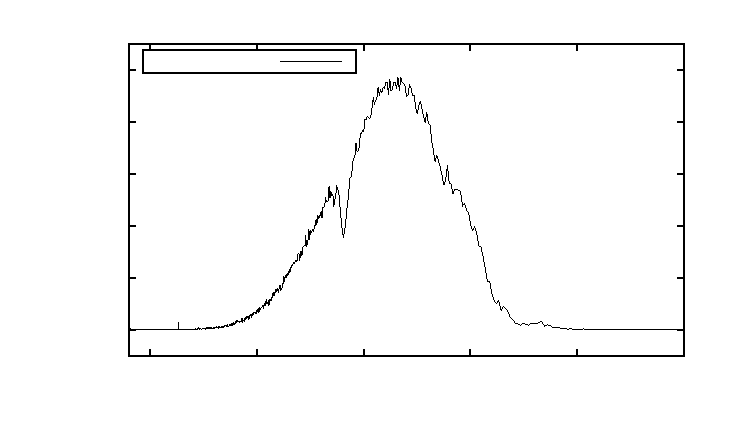
\includegraphics{halo-pbse-spec}}%
    \gplfronttext
  \end{picture}%
\endgroup

				\caption{Spektrum einer Halogenlampe aufgezeichnet mit einem Bleiseleniddetektor 
				sowie $10000$ Samples und $500 \unit{sps}$}
				\label{fig:halo-pbse}
			\end{figure}
		
		% subsubsection gl_hlampenspektrum (end)
	
		\subsubsection{Absorbtionsspektren von Wasser und Benzol} % (fold)
		\label{ssub:absorbtionsspektren_von_wasser_und_benzol}

			Um das Absorptionsverhalten der Substanzen zu Überprüfen wurde zunächst ein möglichst breitbandiges Referenzspektrum erstellt, dazu diente das Halogen-Spektrum aus Abbildung \ref{fig:halo-pbse}.
			Anschließend wurden kleine Proben der Flüssigkeiten in den Strahlengang zwischen Quelle und Kollimator gebracht.
			Das Ergebnis für Wasser ist in Graph \ref{fig:die Henne} gezeigt.
			Wie schon in Abbildung \ref{fig:halo-pbse} sehen wir die Absorption bei $1400 \unit{nm}$.
			Dies deckt sich mit der Referenz aus Anhang \ref{sec:absorptionsspektrum_wasser}.
			Allgemein lässt sich der Verlauf aus \ref{fig:die Henne} als Multiplikation der Spektren von Halogen-Lampe und Wasserdampfabsorption in der Atmosphäre begreifen.
			Für Benzol konnten leider keine verlässlichen Referenzen gefunden werden.
			Auch hier ist der Einbruch bei $1400 \unit{nm}$ zu sehen, der Peak bei ca. $600 \unit{nm}$ gestreutes Licht des Referenzlasers.

			\begin{figure}[htb]
				\centering
				% GNUPLOT: LaTeX picture with Postscript
\begingroup
  \makeatletter
  \providecommand\color[2][]{%
    \GenericError{(gnuplot) \space\space\space\@spaces}{%
      Package color not loaded in conjunction with
      terminal option `colourtext'%
    }{See the gnuplot documentation for explanation.%
    }{Either use 'blacktext' in gnuplot or load the package
      color.sty in LaTeX.}%
    \renewcommand\color[2][]{}%
  }%
  \providecommand\includegraphics[2][]{%
    \GenericError{(gnuplot) \space\space\space\@spaces}{%
      Package graphicx or graphics not loaded%
    }{See the gnuplot documentation for explanation.%
    }{The gnuplot epslatex terminal needs graphicx.sty or graphics.sty.}%
    \renewcommand\includegraphics[2][]{}%
  }%
  \providecommand\rotatebox[2]{#2}%
  \@ifundefined{ifGPcolor}{%
    \newif\ifGPcolor
    \GPcolorfalse
  }{}%
  \@ifundefined{ifGPblacktext}{%
    \newif\ifGPblacktext
    \GPblacktexttrue
  }{}%
  % define a \g@addto@macro without @ in the name:
  \let\gplgaddtomacro\g@addto@macro
  % define empty templates for all commands taking text:
  \gdef\gplbacktext{}%
  \gdef\gplfronttext{}%
  \makeatother
  \ifGPblacktext
    % no textcolor at all
    \def\colorrgb#1{}%
    \def\colorgray#1{}%
  \else
    % gray or color?
    \ifGPcolor
      \def\colorrgb#1{\color[rgb]{#1}}%
      \def\colorgray#1{\color[gray]{#1}}%
      \expandafter\def\csname LTw\endcsname{\color{white}}%
      \expandafter\def\csname LTb\endcsname{\color{black}}%
      \expandafter\def\csname LTa\endcsname{\color{black}}%
      \expandafter\def\csname LT0\endcsname{\color[rgb]{1,0,0}}%
      \expandafter\def\csname LT1\endcsname{\color[rgb]{0,1,0}}%
      \expandafter\def\csname LT2\endcsname{\color[rgb]{0,0,1}}%
      \expandafter\def\csname LT3\endcsname{\color[rgb]{1,0,1}}%
      \expandafter\def\csname LT4\endcsname{\color[rgb]{0,1,1}}%
      \expandafter\def\csname LT5\endcsname{\color[rgb]{1,1,0}}%
      \expandafter\def\csname LT6\endcsname{\color[rgb]{0,0,0}}%
      \expandafter\def\csname LT7\endcsname{\color[rgb]{1,0.3,0}}%
      \expandafter\def\csname LT8\endcsname{\color[rgb]{0.5,0.5,0.5}}%
    \else
      % gray
      \def\colorrgb#1{\color{black}}%
      \def\colorgray#1{\color[gray]{#1}}%
      \expandafter\def\csname LTw\endcsname{\color{white}}%
      \expandafter\def\csname LTb\endcsname{\color{black}}%
      \expandafter\def\csname LTa\endcsname{\color{black}}%
      \expandafter\def\csname LT0\endcsname{\color{black}}%
      \expandafter\def\csname LT1\endcsname{\color{black}}%
      \expandafter\def\csname LT2\endcsname{\color{black}}%
      \expandafter\def\csname LT3\endcsname{\color{black}}%
      \expandafter\def\csname LT4\endcsname{\color{black}}%
      \expandafter\def\csname LT5\endcsname{\color{black}}%
      \expandafter\def\csname LT6\endcsname{\color{black}}%
      \expandafter\def\csname LT7\endcsname{\color{black}}%
      \expandafter\def\csname LT8\endcsname{\color{black}}%
    \fi
  \fi
  \setlength{\unitlength}{0.0500bp}%
  \begin{picture}(6802.00,3968.00)%
    \gplgaddtomacro\gplbacktext{%
      \csname LTb\endcsname%
      \put(946,954){\makebox(0,0)[r]{\strut{} 0}}%
      \put(946,1454){\makebox(0,0)[r]{\strut{} 0.2}}%
      \put(946,1954){\makebox(0,0)[r]{\strut{} 0.4}}%
      \put(946,2453){\makebox(0,0)[r]{\strut{} 0.6}}%
      \put(946,2953){\makebox(0,0)[r]{\strut{} 0.8}}%
      \put(946,3453){\makebox(0,0)[r]{\strut{} 1}}%
      \put(1078,484){\makebox(0,0){\strut{} 400}}%
      \put(2047,484){\makebox(0,0){\strut{} 600}}%
      \put(3015,484){\makebox(0,0){\strut{} 800}}%
      \put(3984,484){\makebox(0,0){\strut{} 1000}}%
      \put(4952,484){\makebox(0,0){\strut{} 1200}}%
      \put(5921,484){\makebox(0,0){\strut{} 1400}}%
      \put(176,2203){\rotatebox{-270}{\makebox(0,0){\strut{}Intensität}}}%
      \put(3741,154){\makebox(0,0){\strut{}Wellenlänge $\lambda \ [\unit{nm}]$}}%
    }%
    \gplgaddtomacro\gplfronttext{%
      \csname LTb\endcsname%
      \put(2398,3530){\makebox(0,0)[r]{\strut{}Messwerte}}%
    }%
    \gplbacktext
    \put(0,0){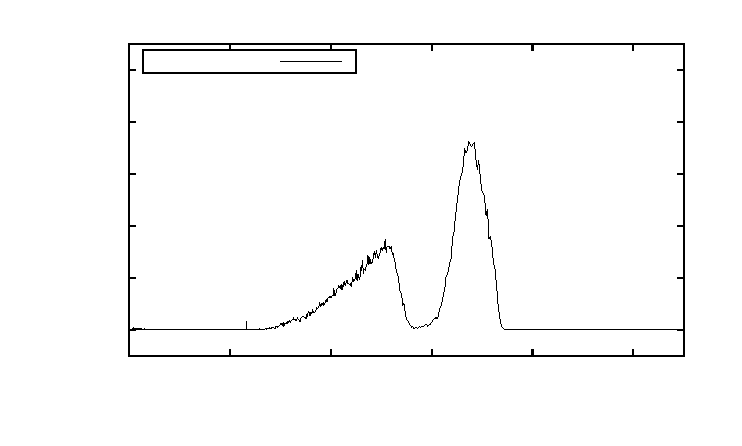
\includegraphics{halo-h20-spec}}%
    \gplfronttext
  \end{picture}%
\endgroup

				\caption{Spektrum einer Halogenlampe nach Durchgang durch $2 \unit{cm}$ Wasser aufgezeichnet mit einem Bleiseleniddetektor 
				sowie $10000$ Samples und $500 \unit{sps}$}
				\label{fig:die Henne}
			\end{figure}
		
			\begin{figure}[htb]
				\centering
				% GNUPLOT: LaTeX picture with Postscript
\begingroup
  \makeatletter
  \providecommand\color[2][]{%
    \GenericError{(gnuplot) \space\space\space\@spaces}{%
      Package color not loaded in conjunction with
      terminal option `colourtext'%
    }{See the gnuplot documentation for explanation.%
    }{Either use 'blacktext' in gnuplot or load the package
      color.sty in LaTeX.}%
    \renewcommand\color[2][]{}%
  }%
  \providecommand\includegraphics[2][]{%
    \GenericError{(gnuplot) \space\space\space\@spaces}{%
      Package graphicx or graphics not loaded%
    }{See the gnuplot documentation for explanation.%
    }{The gnuplot epslatex terminal needs graphicx.sty or graphics.sty.}%
    \renewcommand\includegraphics[2][]{}%
  }%
  \providecommand\rotatebox[2]{#2}%
  \@ifundefined{ifGPcolor}{%
    \newif\ifGPcolor
    \GPcolorfalse
  }{}%
  \@ifundefined{ifGPblacktext}{%
    \newif\ifGPblacktext
    \GPblacktexttrue
  }{}%
  % define a \g@addto@macro without @ in the name:
  \let\gplgaddtomacro\g@addto@macro
  % define empty templates for all commands taking text:
  \gdef\gplbacktext{}%
  \gdef\gplfronttext{}%
  \makeatother
  \ifGPblacktext
    % no textcolor at all
    \def\colorrgb#1{}%
    \def\colorgray#1{}%
  \else
    % gray or color?
    \ifGPcolor
      \def\colorrgb#1{\color[rgb]{#1}}%
      \def\colorgray#1{\color[gray]{#1}}%
      \expandafter\def\csname LTw\endcsname{\color{white}}%
      \expandafter\def\csname LTb\endcsname{\color{black}}%
      \expandafter\def\csname LTa\endcsname{\color{black}}%
      \expandafter\def\csname LT0\endcsname{\color[rgb]{1,0,0}}%
      \expandafter\def\csname LT1\endcsname{\color[rgb]{0,1,0}}%
      \expandafter\def\csname LT2\endcsname{\color[rgb]{0,0,1}}%
      \expandafter\def\csname LT3\endcsname{\color[rgb]{1,0,1}}%
      \expandafter\def\csname LT4\endcsname{\color[rgb]{0,1,1}}%
      \expandafter\def\csname LT5\endcsname{\color[rgb]{1,1,0}}%
      \expandafter\def\csname LT6\endcsname{\color[rgb]{0,0,0}}%
      \expandafter\def\csname LT7\endcsname{\color[rgb]{1,0.3,0}}%
      \expandafter\def\csname LT8\endcsname{\color[rgb]{0.5,0.5,0.5}}%
    \else
      % gray
      \def\colorrgb#1{\color{black}}%
      \def\colorgray#1{\color[gray]{#1}}%
      \expandafter\def\csname LTw\endcsname{\color{white}}%
      \expandafter\def\csname LTb\endcsname{\color{black}}%
      \expandafter\def\csname LTa\endcsname{\color{black}}%
      \expandafter\def\csname LT0\endcsname{\color{black}}%
      \expandafter\def\csname LT1\endcsname{\color{black}}%
      \expandafter\def\csname LT2\endcsname{\color{black}}%
      \expandafter\def\csname LT3\endcsname{\color{black}}%
      \expandafter\def\csname LT4\endcsname{\color{black}}%
      \expandafter\def\csname LT5\endcsname{\color{black}}%
      \expandafter\def\csname LT6\endcsname{\color{black}}%
      \expandafter\def\csname LT7\endcsname{\color{black}}%
      \expandafter\def\csname LT8\endcsname{\color{black}}%
    \fi
  \fi
  \setlength{\unitlength}{0.0500bp}%
  \begin{picture}(6802.00,3968.00)%
    \gplgaddtomacro\gplbacktext{%
      \csname LTb\endcsname%
      \put(946,954){\makebox(0,0)[r]{\strut{} 0}}%
      \put(946,1454){\makebox(0,0)[r]{\strut{} 0.2}}%
      \put(946,1954){\makebox(0,0)[r]{\strut{} 0.4}}%
      \put(946,2453){\makebox(0,0)[r]{\strut{} 0.6}}%
      \put(946,2953){\makebox(0,0)[r]{\strut{} 0.8}}%
      \put(946,3453){\makebox(0,0)[r]{\strut{} 1}}%
      \put(1283,484){\makebox(0,0){\strut{} 500}}%
      \put(2307,484){\makebox(0,0){\strut{} 1000}}%
      \put(3332,484){\makebox(0,0){\strut{} 1500}}%
      \put(4356,484){\makebox(0,0){\strut{} 2000}}%
      \put(5381,484){\makebox(0,0){\strut{} 2500}}%
      \put(6405,484){\makebox(0,0){\strut{} 3000}}%
      \put(176,2203){\rotatebox{-270}{\makebox(0,0){\strut{}Intensität}}}%
      \put(3741,154){\makebox(0,0){\strut{}Wellenlänge $\lambda \ [\unit{nm}]$}}%
    }%
    \gplgaddtomacro\gplfronttext{%
      \csname LTb\endcsname%
      \put(2398,3530){\makebox(0,0)[r]{\strut{}Messwerte}}%
    }%
    \gplbacktext
    \put(0,0){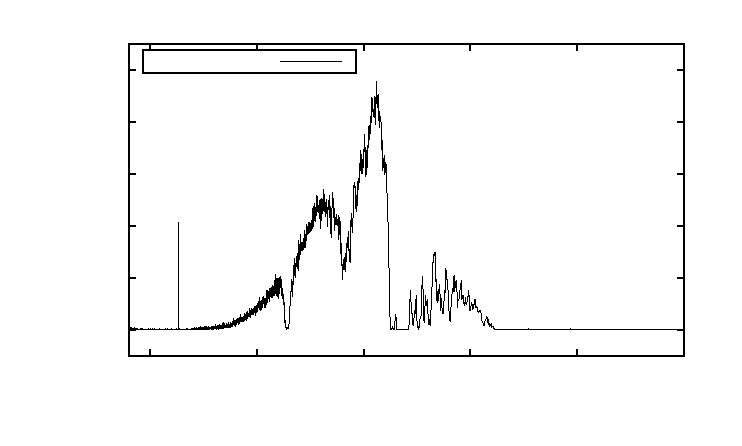
\includegraphics{halo-benz-spec}}%
    \gplfronttext
  \end{picture}%
\endgroup

				\caption{Spektrum einer Halogenlampe nach Durchgang durch $2 \unit{cm}$ Benzol aufgezeichnet mit einem Bleiseleniddetektor 
				sowie $10000$ Samples und $500 \unit{sps}$}
				\label{fig:dich ins Knie}
			\end{figure}

		% subsubsection absorbtionsspektren_von_wasser_und_benzol (end)

	% subsection fourier_spektroskopie (end)

% section messwerte_und_auswertung (end)
	\FloatBarrier
	\null
	\newpage
	\section{Zusammenfassung} % (fold)
\label{sec:zusammenfassung}

	Im Versuch sollten die Analyse von Kristallstrukturen mittels des Drehkristallverfahrens erlernt und angewendet werden.
	Dazu wurden Aufnahmen in den drei Richtungen der $(100)$-, $(110)$- und $(111)$-Achsen angefertigt und vermessen.
	Aus den entstandenen Reflexen konnten nun mittels beugungstheoretischer Grundlagen sowohl Gitterkonstanten als auch die konkrete Kristallstruktur ermittelt werden.
	Die Röntgenfilme zeigten zunächst die erwarteten Eigenschaften.
	Alle Reflexe ließen sich einer konkreten Schichtlinie zuordnen und ihr Abstand bestätigte die theoretischen Formeln.
	Die Auswertung ergab eine fcc-Struktur mit der Gitterkonstanten von LiF.
	Bei genauerer Betrachtung zeigten sich kleine Abweichungen beziehungsweise das mehrfache Auftreten von Reflexen.
	Dies deutet auf leichte Abweichungen in der Kristallstruktur sowie kleinere Fehler bei der Justage der Drehachse hin.
	Um diese zu beheben könnte man die Kristalle kleiner wählen und eventuell eine Nachjustierung anhand der ersten Röntgenaufnahme vornehmen.
	Eine etwas längere Belichtungszeit könnte eventuell auch noch mehr Reflexe hervorbringen beziehungsweise die sehr undeutlichen und schwach ausgeprägten stärker hervorheben.
	Dennoch deckten sich die gemessen Beugungsbilder gut mit den Erwartungen und die vorausgesagten Effekte wie Bragg-Reflexion und Einfluss des Strukturfaktors konnten nachgewiesen werden.
	Die Gegenüberstellung der Aufnahmen mit der Ag-Anode zeigte die Vorzüge eines Metallfilters, da hier die Aufnahmen noch stark mit Bremsstrahlung überlagert waren.
	Durch die veränderten Schichtlinienabstände konnte auf die kleinere Wellenlänge der $K_\alpha$-Linie von Silber in Vergleich zu Kupfer geschlossen werden.
	Auch konnten aus dem Intensitätsverlauf die Abstrahlcharakteristik der Ag-Anode qualitativ nachvollzogen werden.

	Zusammenfassend kann man sagen, dass das Drehkristallverfahren eine einfache und effektive Methode der Festkörperanalyse darstellt, die bei exakter Justage präzise Ergebnisse über Aufbau und Struktur liefern kann.
% section zusammenfassung (end)

	\newpage


	\appendix

	\section{Spektrum - Quecksilberdampflampe} % (fold)
	\label{sec:hg_spektrum}
	
		\begin{figure}[h]
			\centering
			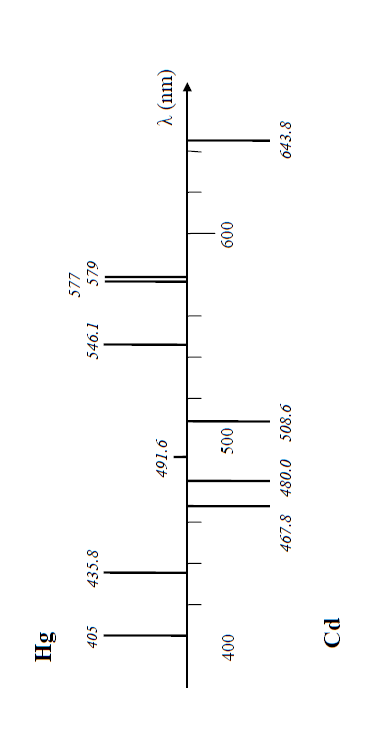
\includegraphics[scale = 0.75]{images/hg-cd-reference.PNG}
			\caption{bekanntes Spektrum der Quecksilberdampflampe \\ Quelle: Versuchsanleitung Sonnenspektroskopie}
			\label{fig:hg-ref}
		\end{figure}

	% section hg_spektrum (end)

	\FloatBarrier
	\newpage

	\section{Absorptionsspektrum Wasser} % (fold)
	\label{sec:absorptionsspektrum_wasser}
	
		\begin{figure}[htb]
			\centering
			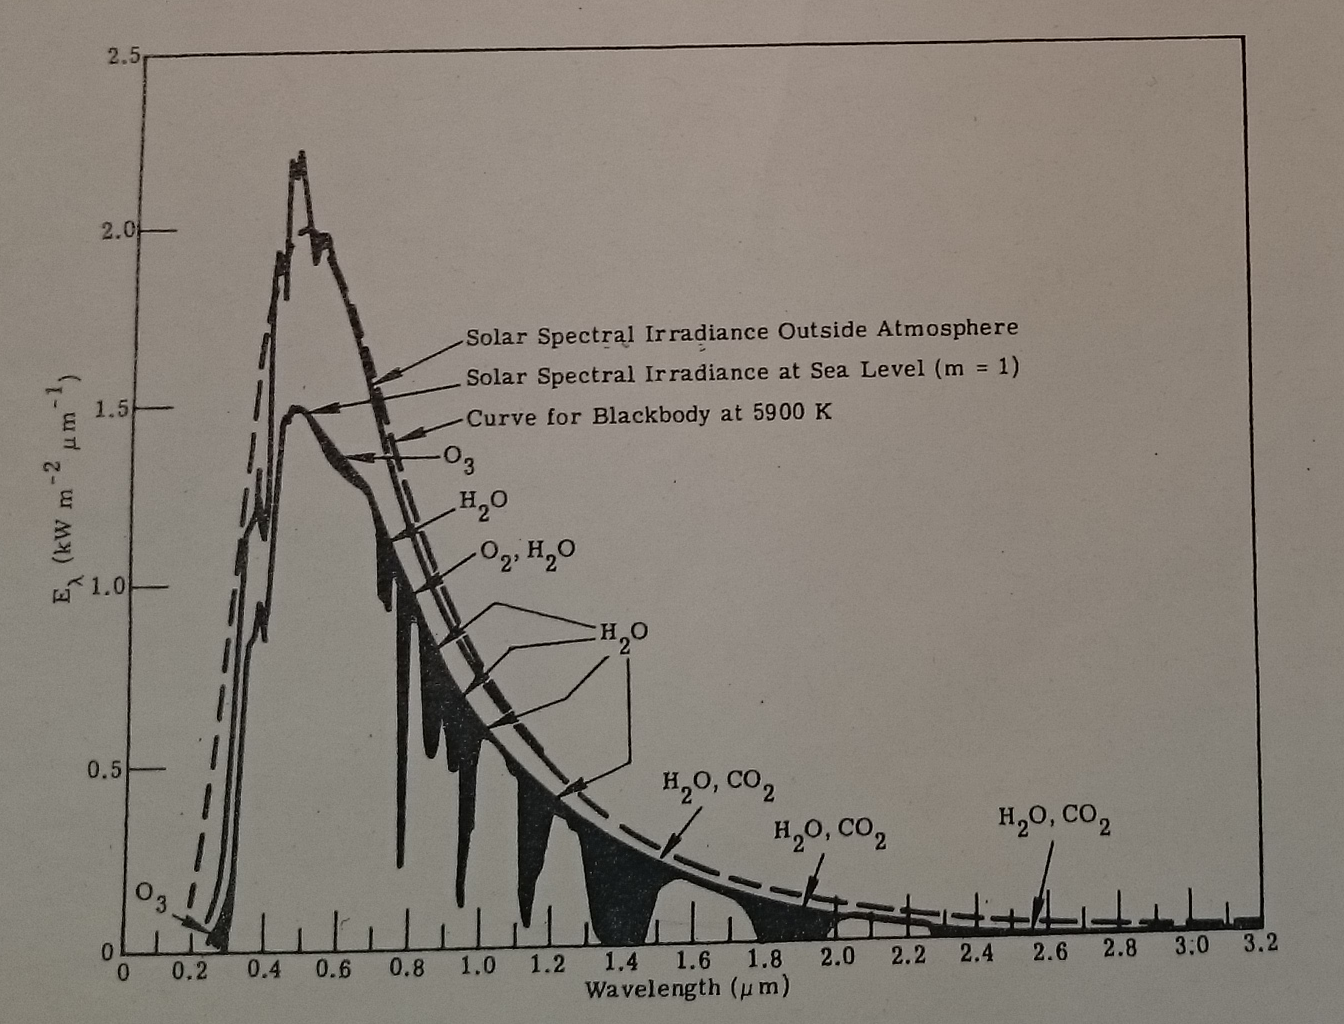
\includegraphics[scale=0.25]{images/h2o-spec.png}
			\caption{Absorbtionsspektrum des Wassers \\ Quelle: Versuchsunterlagen}
			\label{fig:}
		\end{figure}

	% section absorptionsspektrum_wasser (end)

	\FloatBarrier

	\newpage
	\pagestyle{empty}
	\topskip0pt
	\vspace*{\fill}
	\centering $\mathscr{D}$anke für die $\mathscr{K}$ekse!
	\vspace*{\fill}

\end{document}